% !TEX root = ../diz.tex
In this chapter we propose various modifications of sequential P systems and study their effect on computing power and decidability of behavioral properties.

We have presented the current state of the research of the P system variants. Especially the parallelism options have been investigated very well, but there are still some gaps that should be filled. For many variants the universality has been proven only when working in the maximally parallel mode. In most cases the sequential mode is strictly weaker, but this is not always true.

We have studied several variants of sequential P systems in terms of computational power and decision power of behavioral properties. Two of these results have appeared as a contribution on the Computability in Europe conference series.

\section{Inhibitors} % (fold)
\label{sec:inhibitors}
% !TEX root = ../diz.tex
A sequential variant without priorities and with cooperative rules is not universal (see \cite{Ibarra04dang}). They have tried modifying the variant to increase the computational power and showed that with rules for membrane creation with unbounded number of membranes it became universal.

We have tried another approach using rules with inhibitors. This variant is computationally complete in both generating and accepting case. For the generative case we present a proof by a simulation of maximal parallel P system and in the accepting case we prove it can simulate a register machine.

Original definition of P systems with inhibitors (see \cite{Ionescu:jucs_10_5:on_p_systems_with}) allow to use only one inhibitor per rule, e.g. $u\rightarrow v|_{\neg i}$. Alternative definition (see \cite{Agrigoroaiei:2010:Dissolution}) allow to use whole inhibitor set in the rule like $u\rightarrow v|_{\neg B}$, where $B$ is a set of objects. Such a rule can be applied only if no element of $B$ is present in the region.

For sequential P systems, the following lemma will show the equivalence of these definitions for our setting. However, a special condition must be fulfilled, the regions with such rules cannot be empty.

% !TEX root = ../diz.tex
\begin{lemma}
\label{lemma:inhibitor_step}
  If there is at least one object present in each region of a P system, rewriting step in P system with inhibitor set can be simulated by multiple consecutive steps of P system with single inhibitor.
\end{lemma}

\begin{dokaz}
  Consider a P system with the alphabet $\Sigma$.
  For each rule $u\rightarrow v|_{\neg B}$, where $B=\{b_1, b_2, \dots ,b_n\}$ we will have rules:
    \begin{align*}
      c\rightarrow&c|GONE_{b}|_{\neg b} \text{~for all~} c\in \Sigma, b\in B \\
      u|GONE_{b_1}|GONE_{b_2}|\dots|GONE_{b_n}\rightarrow&v|GONE_{b_1}|GONE_{b_2}|\dots|GONE_{b_n}
    \end{align*}

\end{dokaz}

Note that symbols $GONE_b$ are created automatically when some object $c$ is present in the region. 

\begin{veta}
  The sequential P system with inhibitors defines the same Parikh image of language as P system with maximal parallelism.
\end{veta}

\begin{dokaz}
  We show that we can simulate maximal parallel step of P system with several steps of sequential P system with inhibitors. The proof is quite technical with some workarounds.

  % Membrane states

  It is important to note that in the maximal parallel step the rewriting occurs in all membranes, so we need to synchronize this process. Every membrane will have a state, represented as an object.

  The $RUN$ state represents that the rewriting still occurs. When there are no more rules to apply, the region has done its maximal parallel step and proceeds to the state $SYNCHRONIZE$. Other states are just technical - we need to implement sending objects between membranes and preparing for the next maximal parallel step by unmarking newly created objects in the current maximal parallel step, which have been marked to prevent double rewriting in one step.

  \begin{itemize}
    \item $RUN$: Rewriting occurs. Objects that are to be sent to the parent membrane are directly sent because the parent membrane is already in $RUN$ or $SYNCHRONIZE$ phase, so the $a^{\prime}$ symbols that are sent don't break anything. But objects that are to be sent down, cannot be sent immediately because child membranes can be in the previous phase waiting to restore symbols from previous step. Current symbols could interfere with them and be rewritten twice in this step. Such objects are only marked as ``to be sent down'': $a^{\downarrow\prime}$

    \item $SYNCHRONIZE$: Rewriting has ended and the membrane is waiting to get signal $SYNCED$ from the parent membrane to continue to the next step.

    \item $SENDDOWN$: Signal $SYNCED$ was caught and now all descendant membranes are in $SYNCHRONIZE$ phase so $a^{\downarrow\prime}$ can be sent down.

    \item $RESTORE$: All $a^{\prime}$ symbols are being restored to $a$, so the next step of rewriting can take place.
  \end{itemize}

  % Rewriting rules

  \begin{itemize}
    \item For every rule $r_i\in R$ such that
      \begin{align*}
        r_i = a_1^{M(a_1)}a_2^{M(a_2)}\dots a_n^{M(a_n)} \rightarrow a_1^{N(a_1)}a_2^{N(a_2)}\dots a_n^{N(a_n)}
      \end{align*}
      we will have the following rules:
      \begin{align*}
        &a_1^{M(a_1)-m_1}\dot{a}_1^{m_1}
        a_2^{M(a_2)-m_2}\dot{a}_2^{m_2}\dots
        a_n^{M(a_n)-m_n}\dot{a}_n^{m_n}|RUN \\
        \rightarrow &a_1^{\prime N(a_1)}a_2^{\prime N(a_2)}\dots a_n^{\prime N(a_n)}|RUN
      \end{align*}
      
      There will be such rule for each $0\leq m_i\leq M(a_i)$. It represents the idea that $\dot{a}$ can be used in rewriting in the same way as $a$. Right side of the rules contains symbols $a^\prime$, that prevents the symbols to be rewritten again.

    \item For every symbol $a\in V$ we will have the following rules:

    $a|RUN \rightarrow \dot{a}|RUN|_{\neg \dot{a}}$

    There will be at most one occurrence of $\dot{a}$.

    \item For every rule $r_i\in R$ there will be a rule that detects if the rule $r_i$ is not applicable. According to left side of the rule $r_i$, symbol $UNUSABLE_i$ will be created when there is not enough objects to fire the rule $r_i$. It means that left side of rule $r_i$ requires more instances of some object than are present in membrane.

    If the left side is of type:
    \begin{itemize}
      \item $a$: It is a context free rule. The rule can't be used if there is no occurrence of $a$ nor $\dot{a}$.

      $RUN \rightarrow UNUSABLE_i|RUN|_{\neg\{UNUSABLE_i, a, \dot{a}\}}$

      \item $ab$: It is a cooperative rule with two distinct objects on the left side. The rule cannot be used if there is one of them missing.

      $RUN \rightarrow UNUSABLE_i|RUN|_{\neg\{UNUSABLE_i, a, \dot{a}\}}$

      $RUN \rightarrow UNUSABLE_i|RUN|_{\neg\{UNUSABLE_i, b, \dot{b}\}}$

      \item $a^2$: It is a cooperative rule with two same objects. The rule can't be used if there is at most one occurrence of the symbol. That happens if there is no occurrence of $a$. There can still be $\dot{a}$, but at most one occurrence.

      $RUN \rightarrow UNUSABLE_i|RUN|_{\neg\{UNUSABLE_i, a\}}$
    \end{itemize}

    \item For every membrane with label $i$ there will be a rule:
    \begin{align*}
      &UNUSABLE_1|UNUSABLE_2|\dots|UNUSABLE_m|RUN \\
      \rightarrow &SYNCHRONIZE|SYNCTOKEN_i\uparrow
    \end{align*}

    If no rule can be used, maximal parallel step in the region is completed hence it goes to the synchronization phase and sends a synchronization token to the parent membrane.

    \item For every membrane there will be a rule:
    \begin{align*}
      &SYNCHRONIZE|SYNCTOKEN_j \\
      \rightarrow &SYNCHRONIZE|SYNCTOKEN_j\uparrow
    \end{align*}

    Membrane resends all synchronization tokens from child membranes to the parent membrane.

    \item In the skin membrane there is a rule which collects all the synchronization tokens from all membranes $1\dots k$ and then sends down signal that synchronization is complete. But before that, there can be some symbols that should be sent down, but they weren't, because the region below could have not started the rewriting phase that time. The result was just marked with $a^{\downarrow\prime}$.
    \begin{align*}
      &SYNCTOKEN_1|\dots|SYNCTOKEN_k|SYNCHRONIZE \\
      \rightarrow &SENDDOWN
    \end{align*}

    \item Every membrane other than skin membrane have to receive the signal to go to the senddown phase:

    $SYNCHRONIZE|SYNCED \rightarrow SENDDOWN$

    \item Every membrane will have rules for every symbol $a\in V$ to send down all unsent objects that should have been sent down:

    $SENDDOWN|a^{\downarrow\prime} \rightarrow SENDDOWN|a^{\prime}\downarrow$

    \item Every membrane will have a rule for detecting when all such objects have been sent and it goes to restore phase:

    $SENDDOWN \rightarrow RESTORE|_{\neg \{a_i^{\downarrow\prime}|1\leq i\leq n\}}$

    \item In the restore phase all symbols $a^{\prime}$ will be rewritten to $a$ in order to be able to be rewritten in the next maximal parallel step:

    $RESTORE|a^{\prime} \rightarrow RESTORE|a$
    
    \item When using lemma~\ref{lemma:inhibitor_step}, there may be some $GONE$ symbols left and now is the time to clear them:

    $RESTORE|GONE_i \rightarrow RESTORE$

    \item When the restore phase ends, it sends down a signal that all membranes have been already synchronized and next phase of rewriting has began in upper membranes:

    $RESTORE \rightarrow RUN|SYNCED\downarrow|_{\neg \{a_i^{\prime}|1\leq i\leq n\}\cup\{GONE_i|1\leq i\leq n\}}$
  \end{itemize}

  \definecolor{run}{rgb}{1,0.5,0}
  \definecolor{restore}{rgb}{0,0.5,0}
  \definecolor{synchronize}{rgb}{0,0,1}
  \definecolor{senddown}{rgb}{1,0,0}
  % Narrow texts in boxes
  \providecommand{\narrow}[1]{\scalebox{.85}[1.0]{#1}}

  \begin{figure}
    \def\svgwidth{\textwidth}
    \input{possible_pairs_of_states_of_parent_and_child_membrane.pdf_tex}
    % 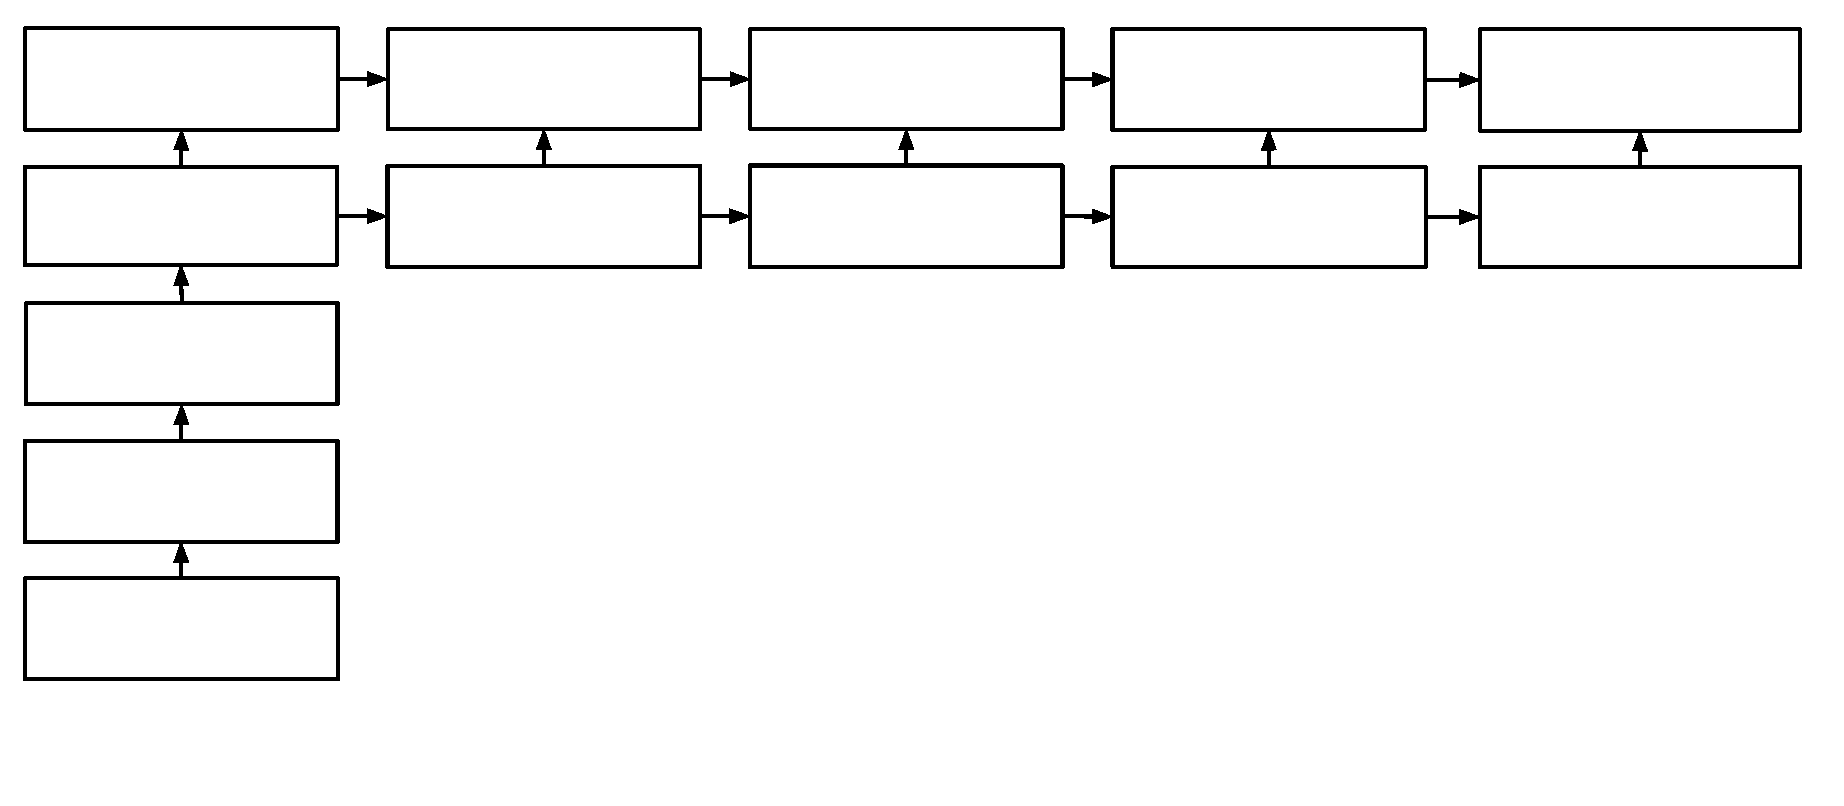
\includegraphics[width=\textwidth]{possible_pairs_of_states_of_parent_and_child_membrane}
    \caption{Possible pairs of states of parent and child membrane}
    \label{fig:possible_pairs_of_states_of_parent_and_child_membrane}
  \end{figure}

  \begin{figure}
    \def\svgwidth{\textwidth}
    \input{snapshot_of_all_membrane_states_while_simulating.pdf_tex}
    % 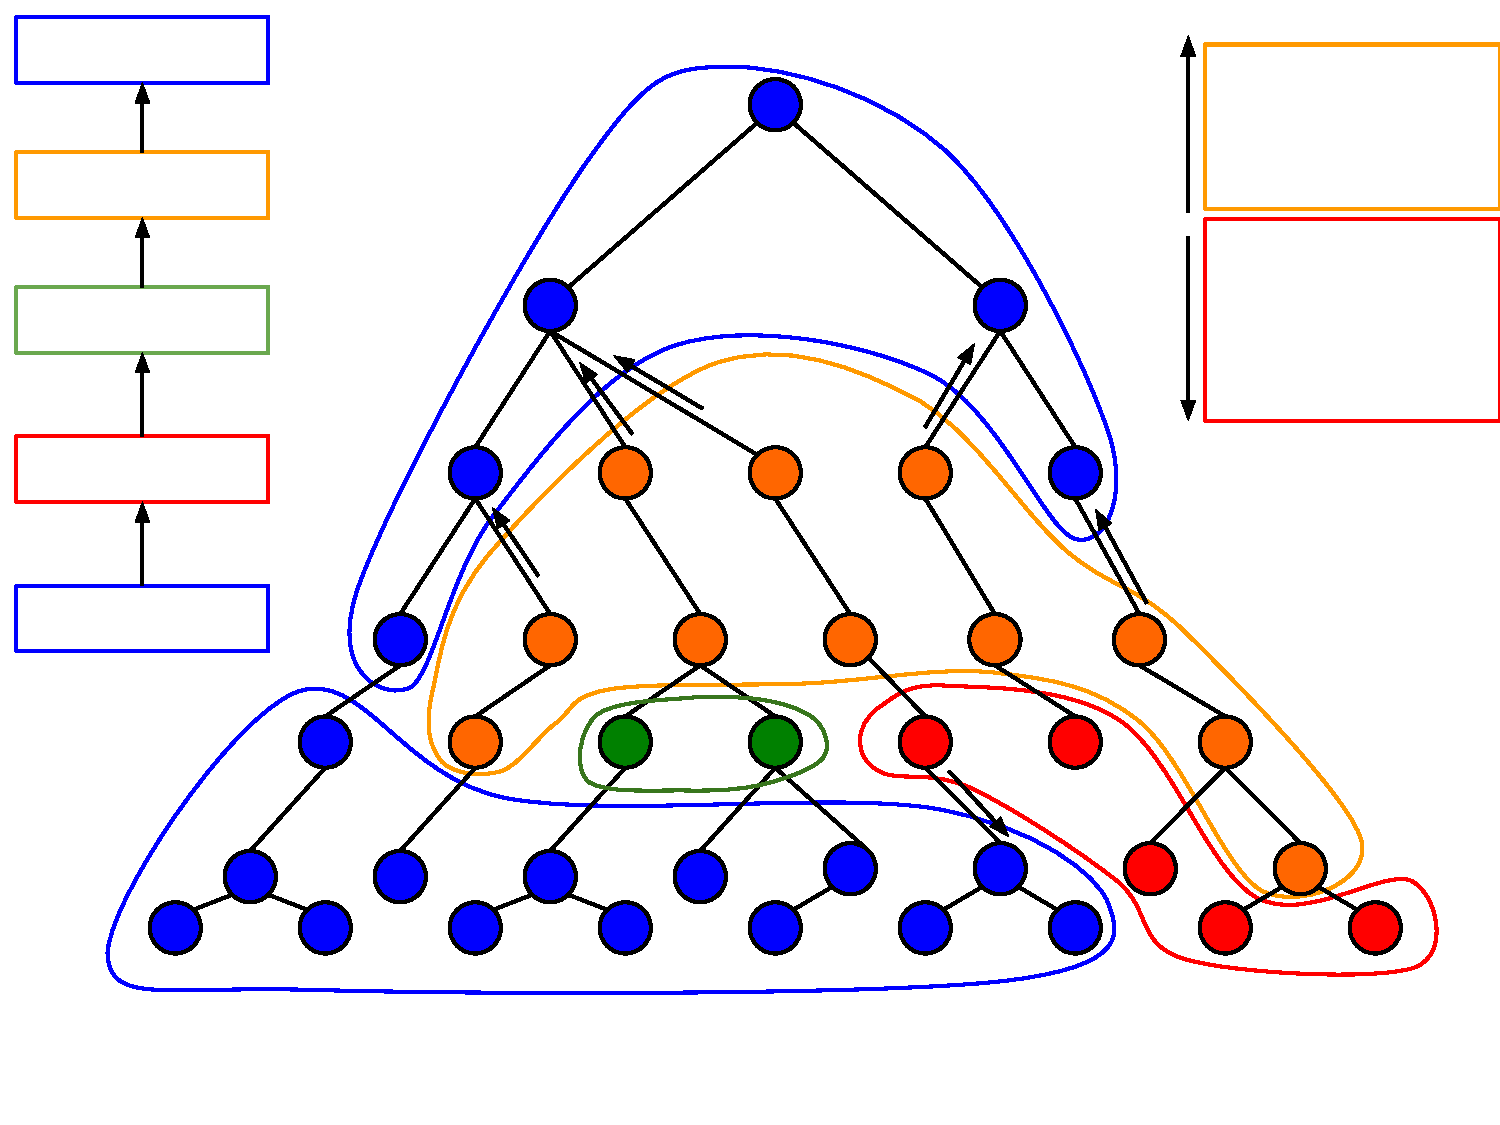
\includegraphics[width=\textwidth]{snapshot_of_all_membrane_states_while_simulating}
    \caption{Snapshot of all membrane states while simulating}
    \label{fig:snapshot_of_all_membrane_states_while_simulating}
  \end{figure}

  The pairs of possible phases of the parent and child membrane are shown in the figure \ref{fig:possible_pairs_of_states_of_parent_and_child_membrane} along with transitions between two consecutive global synchronizations - after the maximal parallel steps $i$ and $i+1$.

  In the figure \ref{fig:snapshot_of_all_membrane_states_while_simulating} the membrane structure is presented as a hierarchical structure. Every membrane is in one of four phases. It can be seen that the sending of the objects is performed in such phases that the receiving membrane is in either $RUN$ or $SYNCHRONIZE$ phase, so the received objects (marked $a^\prime$) does not interfere with rewriting.

  Another interesting idea can be seen in the figure \ref{fig:snapshot_of_all_membrane_states_while_simulating} that when a region is in the $SENDDOWN$ phase and objects are sent through the child membrane, the receiving region is in the $SYNCHRONIZE$ phase waiting for the $SYNCED$ signal, which will be sent to it when $SENDDOWN$ and $RESTORE$ phases finished.

  All membranes are nonempty during the simulation because at least the object representing the current phase is always present. By lemma~\ref{lemma:inhibitor_step} the rules with set of inhibitors can be simulated by single inhibitors.


\end{dokaz}




We have also reached this result in the accepting case by simulation of register machines.

% !TEX root = ../diz.tex
\begin{veta}
  Sequential P systems with cooperative rules and inhibitors can simulate register machines and thus equal $PsRE$.
\end{veta}


\begin{dokaz}
\label{proof:reg_by_inh}
  Suppose we have an $n$-register machine $M = (n,P,i,h)$. In our simulation we will have a membrane structure consisting of single membrane and the contents of register $j$ will be represented by the multiplicity of the object $a_j$.

  We will simulate the register machine by P system $(\Sigma, \mu, w, R)$, where:
  \begin{itemize}
    \item $\Sigma$ is an alphabet consisting of symbols that represent registers $a_1,\dots a_n$, instruction labels from the register machine $M$ and a halting symbol $\#$,
    \item $\mu$ is a membrane structure consisting of one single membrane,
    \item $w$ is initial contents of the membrane. It contains symbols for the input for the machine $a_i^{n_i}$ where $n_i$ is initial state of register with label $i$ and initial instruction label $e$.
    \item $R$ is a set of rules in the skin membrane.
  \end{itemize}
    
  For all instructions of type $(e : add(j), k, l)$ we will have rules:
  \begin{align*}
    e \rightarrow a_j|k\\
    e \rightarrow a_j|l.
  \end{align*}

  For all instructions of type $(e : sub(j), k, l)$ we will have rules:
  \begin{align*}
    e|a_j \rightarrow k\\
    e \rightarrow l|_{\neg a_j}.
  \end{align*}

  And finally halting rules:
  \begin{align*}
    h|a_j \rightarrow h|\#\text{~for all~}a\leq j\leq n,\\
    \# \rightarrow \#.
  \end{align*}

  For a configuration $(j, m_1, \dots, m_n)$ of the simulated register machine $M$ the skin membrane of the simulating P system contains a symbol $j$ and objects representing contents of registers $a_1^{m_1}, \dots, a_n^{m_n}$.

  When the halting instruction is reached, if there is an object present in the membrane, the hash symbol $\#$ is created and the rule $\# \rightarrow \#$ will be applicable forever as there is no rule to remove the symbol $\#$. If there is no object present, there is no rule to apply and computation will halt. It corresponds to the condition that all registers should be empty when halting. \qed
\end{dokaz}

\subsection{Concluding remarks} % (fold)
\label{sub:concluding_remarks_of_inhibitors}

Future plans include research other more restricted variants such as omitting cooperation in the rules or restrict the power of inhibitors.

% subsection concluding_remarks (end)

% section inhibitors (end)

\section{Active membranes} % (fold)
\label{sec:active_membranes}
In this section we study a variant of sequential systems where universality can be achieved without checking for zero by allowing membranes to be created unlimited number of times \cite{Ibarra05Active}. Such P systems are called active P systems. Contrary, if we place a limit on the number of times a membrane is created, we get a class of P systems which is only equivalent to vector addition systems, hence not universal.

In Subsection \ref{sub:active_p_systems} we will introduce membrane structure and formally define membrane configuration and active P system, because standard definitions are not convenient for our formal proofs.

The Subsection \ref{sub:termination_problems} contains two main results. The existence of an infinite computation is surprisingly\footnote{At first sight it seems to relate to the Rice's theorem, but it is not the case.} shown to be decidable.
On the other hand, the existence of a halting computation is shown to be undecidable.

\subsection{Active P systems} % (fold)
\label{sub:active_p_systems}

\begin{definition}
  \label{def:membrane_structure}
  Let $\Sigma$ be a set of objects. We denote by $\mathbb N^\Sigma$ a set of all mappings from $\Sigma$ to $\mathbb N$, so it contains all multisets of objects from $\Sigma$. A {\bf membrane configuration} is a tuple $(T, l, c)$, where:
  \begin{itemize}
    \item $T$ is a rooted tree,
    \item $l\in\mathbb N^{V(T)}$ is a mapping that assigns for each node of $T$ a number (label), where $l(r_T)=1$, so the skin membrane is always labeled with 1,
    \item $c\in(\mathbb N^\Sigma)^{V(T)}$ is a mapping that assigns for each node of $T$ a multiset of objects from $\Sigma$, so it represents the contents of the membrane.
  \end{itemize}
\end{definition}

\begin{definition}
  \label{def:active_p_system}
  An {\bf active P system} is a tuple $(\Sigma, C_0, R_1, R_2, \ldots , R_m)$, where:
  \begin{itemize}
    \item $\Sigma$ is a set of objects,
    \item $C_0$ is initial membrane configuration,
    \item $R_1,R_2,\ldots R_m$ are finite sets of rewriting rules associated with the labels $1,2,\ldots,m$ and can be of forms:
    \begin{itemize}
      \item $u\rightarrow w$, where $u\in \Sigma^+$, $w\in (\Sigma\times\{\cdot, \uparrow, \downarrow_j\})^*$ and $1\leq j\leq m$,
      \item $u\rightarrow w\delta$, where $u\in \Sigma^+$, $w\in (\Sigma\times\{\cdot, \uparrow, \downarrow_j\})^*$ and $1\leq j\leq m$,
      \item $u\rightarrow [_j v]_j$, where $u\in \Sigma^+, v\in \Sigma^*$ and $1\leq j\leq m$.
    \end{itemize}
  \end{itemize}
\end{definition}

Although rewriting rules are defined as strings, $u,v$ and $w$ represent multisets of objects from $\Sigma$. For the first two forms, each rewriting rule may specify for each object on the right side, whether it stays in the current region (we will omit the symbol $\cdot$), moves through the membrane to the parent region ($\uparrow$)
or to a specific child region ($\downarrow_j$, where $j$ is a label of a membrane). If there are more child membranes with the same label, one is chosen nondeterministically.
We denote these transfers with an arrow immediately after the symbol.
An example of such rule is the following: $abb\rightarrow ab\downarrow_2 c\uparrow c\delta$.
Symbol $\delta$ at the end of the rule means that after the application of the rule, the membrane is dissolved and its contents (objects, child membranes) are propagated to the parent membrane.
Active P systems differ from classic (passive) P systems in ability to create new membranes by rules of the third form. Such rule will create new child membrane with a given label $j$ and a given multiset of objects $v$ as its contents.

% applicable rule definition

\begin{definition}
  \label{def:applicable_rule_of_active_p_system}
  For an active P system $(\Sigma, C_0, R_1, R_2, \ldots , R_m)$, configuration $C = (T, l, c)$, membrane $d\in V(T)$ the rule $r\in R_{l(d)}$ is {\bf applicable} iff:
  \begin{itemize}
    \item $r = u\rightarrow w$ and $u\subseteq c(d)$ and for all $(a,\downarrow_k)\in w$ there exists $d_2\in V(T)$ such that $l(d_2)=k \wedge parent(d_2) = d$,
    \item $r = u\rightarrow w\delta$ and $u\subseteq c(d)$ and for all $(a,\downarrow_k)\in w$ there exists $d_2\in V(T)$ such that $l(d_2)=k \wedge parent(d_2) = d$ and $d\neq r_T$,
    \item $r = u\rightarrow [_j v]_j$ and $u\subseteq c(d)$.
  \end{itemize}
\end{definition}

In this section we assume only sequential systems, so in each step of the computation, there is one rule nondeterministically chosen among all applicable rules in all membranes to be applied as already stated in the definition \ref{def:computation_step_of_a_sequential_P_system}.

% subsection active_p_systems (end)

\subsection{Active membranes with a limit on the total number of membranes} % (fold)
\label{sub:active_membranes_with_a_limit_on_total_number_of_membranes}

For the simplicity of proofs it is convenient to introduce a variant with a global limit upon the membrane structure. We achieve this by restricting the rule application such that if the rule would result in a structure exceeding the limit, the rule will not be applicable.

\begin{definition}
  \label{def:active_p_system_with_a_limit_on_total_number_of_membranes}
  An {\bf active P system with a limit on the total number of membranes} is a tuple $\Pi = (\Sigma, L, C_0, R_1, R_2, \ldots , R_m)$, where:
  \begin{itemize}
    \item $(\Sigma, C_0, R_1, R_2, \ldots , R_m)$ is an active P system from the definition \ref{def:active_p_system},
    \item $L\in \mathbb N$ is a limit on thetotal number of membranes.
  \end{itemize}
\end{definition}
Anytime during the computation, a configuration $(T, l, c)$ is not allowed to have more than $L$ membranes, so the following invariant holds: $|V(T)|\leq L$.
This is achieved by adding a constraint for rule of the form $r = u\rightarrow [_k v]_k$, which is defined to be applicable iff $u\subseteq c(d)$ and $|V(T)|<L$. If the number of membranes is equal to $L$, there is no space for newly created membrane, so in that case such rule is not applicable.

\begin{definition}
  \label{def:applicable_rule_of_active_p_system_with_a_limit_on_total_number_of_membranes}
  For active P system with a limit on the total number of membranes $(\Sigma, L, C_0, R_1, R_2, \ldots , R_m)$, configuration $C = (T, l, c)$, membrane $d\in V(T)$ the rule $r\in R_{l(d)}$ is {\bf applicable} iff:
  \begin{itemize}
    \item $r = u\rightarrow w$ and $u\subseteq c(d)$ and $\forall (a,\downarrow_k)\in w \exists d_2\in V(T): l(d_2)=k \wedge parent(d_2) = d$,
    \item $r = u\rightarrow w\delta$ and $u\subseteq c(d)$ and $\forall (a,\downarrow_k)\in w \exists d_2\in V(T): l(d_2)=k \wedge parent(d_2) = d$ and $d\neq r_T$,
    \item $r = u\rightarrow [_j v]_j$ and $u\subseteq c(d)$ and $|V(T)|<L$.
  \end{itemize}
\end{definition}

% subsection active_membranes_with_a_limit_on_total_number_of_membranes (end)

\subsection{Termination problems} % (fold)
\label{sub:termination_problems}

In this subsection we recall the halting problem for Turing machines. The problem is to determine, given a deterministic Turing machine and an input, whether the Turing machine running on that input will halt. It is one of the first known undecidable problems. On the other hand, for non-deterministic machines, there are two possible meanings for halting. We could be interested either in:
\begin{itemize}
  \item whether there exists an infinite computation (the machine can run forever), or
  \item whether there exists a finite computation (the machine can halt).
\end{itemize}

We can ask the same questions for non-deterministic P systems.
For example we can look at the P system from the figure \ref{fig:a_single_membrane_sample_p_system}. Its computation tree (figure \ref{fig:computation_tree}) contains an infinite branch, so there exists an infinite computation with rule $r_1$ applied in each step. There is also a finite branch, so there exists a finite computation, e.g. applying rule $r_2$ results in a halting configuration.

\begin{figure}
  \centering
  \begin{minipage}{.4\textwidth}
    \begin{tikzpicture}[node distance=2mm,-triangle 45,line width=1mm]
      \tikzstyle{label of} = [above left=-5mm of #1]
      \tikzstyle{membrane} = [draw,thick,rounded corners=1cm,minimum width=2cm,minimum height=2cm,rectangle]
      \node [membrane] (m1) {
        \begin{minipage}{.8\textwidth}
          \begin{align*}
            a\\
            r_1: a\rightarrow a\\
            r_2: a\rightarrow b\\
          \end{align*}
        \end{minipage}
      };
    \end{tikzpicture}
    \captionof{figure}{A single-membrane sample P system}
    \label{fig:a_single_membrane_sample_p_system}
  \end{minipage}
  \hspace{.08\textwidth}
  \begin{minipage}{.5\textwidth}
    \centering
    \begin{tikzpicture}[level distance=2cm,sibling distance=4cm,-triangle 45]
      \tikzstyle{every node} = [circle,draw]
      \node (Root) {a}
        child {
          node {a}
          child {
            node [draw=none] {$\ldots$}
            edge from parent node [above left,draw=none] {$r_1$}
          }
          child { node {b} edge from parent node [above right,draw=none] {$r_2$} }
          edge from parent node [above left,draw=none] {$r_1$}
        }
        child { node {b} edge from parent node [above right,draw=none] {$r_2$} };
    \end{tikzpicture}  
    \captionof{figure}{The computation tree of the P system from the figure \ref{fig:a_single_membrane_sample_p_system}}
    \label{fig:computation_tree}
  \end{minipage}
\end{figure}

We will prove the (un)decidability of these problems on active P systems with limit on the total number of membranes. The results are quite interesting, because:

\begin{veta}
  Sequential active P systems with limit on the total number of membranes are universal.
\end{veta}

\begin{dokaz}
  The proof of this theorem for sequential active P systems in \cite{Ibarra05Active} uses simulation of register machines and during the simulation, every configuration has at most three membranes. Hence the active P system with limit on the total number of membranes exists (e.g. with $L=3$), so the universality holds.
  \qed
\end{dokaz}

\subsubsection{Existence of infinite computation} % (fold)
\label{ssub:existence_of_infinite_computation}

We will propose an algorithm for deciding existence of infinite computation. Basic idea is to consider the minimal coverability graph (\cite{Rozenberg93MinimalCoverabilityGraph}), where nodes are configurations and an edge leads from the configuration $C_1$ to the configuration $C_2$, whenever there is a rule applicable in $C_1$, which results in $C_2$. The construction in \cite{Rozenberg93MinimalCoverabilityGraph} is performed on Petri nets, where the configuration consists just of a vector of natural numbers. The situation is the same for single-membrane sequential P systems. We need to modify the construction for active P systems.

\begin{definition}
  A configuration $C_2 = (T_2, l_2, c_2)$ {\bf covers} configuration $C_1 = (T_1, l_1, c_1)$ iff $\exists$ isomorphism $f: T_1\rightarrow T_2$ preserving membrane labels and contents: $\forall d\in T_1$ the following properties hold: $l_1(d)=l_2(f(d))\wedge c_1(d)\subseteq c_2(f(d))$. We will denote this with $C_1\leq C_2$.
\end{definition}

\begin{figure}
  \begin{tikzpicture}[node distance=2mm,line width=1mm]
    \tikzstyle{label of} = [above left=-5mm of #1]
    \tikzstyle{membrane} = [draw,thick,rounded corners=1cm,minimum width=2cm,minimum height=2cm,rectangle]
    \node [membrane] (m1) {
      \begin{minipage}{.42\textwidth}
        \begin{align*}
          a\\
        \end{align*}
      \end{minipage}
    };
    \node [label of=m1] (l1) {1};
    \node [below=1mm of m1] (c1) {$C_1$};
    \node [membrane,right=.08\textwidth of m1] (m2) {
      \begin{minipage}{.42\textwidth}
        \begin{align*}
          a,b\\
        \end{align*}
      \end{minipage}
    };
    \node [label of=m2] (l2) {1};
    \node [below=1mm of m2] (c2) {$C_2$};
    \node [membrane,below=.08\textwidth of c1] (m3) {
      \begin{minipage}{.42\textwidth}
        \begin{align*}
          a\\
        \end{align*}
      \end{minipage}
    };
    \node [label of=m3] (l3) {2};
    \node [below=1mm of m3] (c3) {$C_3$};
    \node [membrane,below=.08\textwidth of c2] (m4) {
      \begin{tikzpicture}
        \node (m4a) {$a$};
        \tikzstyle{label of} = [above left=-15mm of #1]
        \node [membrane,minimum width=3cm,right=1mm of m4a] (m5) {a};
        \node [label of=m5] (l5) {1};
      \end{tikzpicture}      
    };
    \node [label of=m4] (l4) {1};
    \node [below=1mm of m4] (c4) {$C_4$};
  \end{tikzpicture}
  \caption{Sample membrane configurations}
  \label{fig:sample_membrane_configurations}
\end{figure}

\begin{example}
  In the figure \ref{fig:sample_membrane_configurations} there are four membrane configuration. $C_1\leq C_2$, because the membrane structures consists of one membrane, so the corresponding trees are isomorphic. The label is the same and the contents of the membrane in $C_1$ is a subset of the contents of the membrane in $C_2$. It does not have to be a proper subset, i.e. $C_1\leq C_1$.$C_1$ and $C_3$ are incomparable, because the label is different, so neither $C_1\leq C_3$ nor $C_3\leq C_1$ holds. $C_1$ and $C_4$ are also incomparable, because the trees of their membrane structure are not isomorphic.
\end{example}

We will now follow with a proof of an important property of the covering relation - that it maintains rule applicability.

\begin{lemma}
\label{rule_applicability_lemma}
  For sequential active P system with limit on the total number of membranes, if $C_2 = (T_2, l_2, c_2)$ {\bf covers} configuration $C_1 = (T_1, l_1, c_1)$, then there is an isomorphism $f: T_1\rightarrow T_2$ such that if a rule $r$ is applicable in membrane $d\in T_1$, then $r$ is applicable in $f(d)$.
\end{lemma}

\begin{dokaz}
  Suppose $r$ is applicable in $d$. Then the left side $u$ of the rule $r$ is contained within the contents of the membrane $u\subseteq c_1(d)$. Because $C_1\leq C_2$, then there is an isomorphism $f:T_1\rightarrow T_2$ such that $c_1(d)\subseteq c_2(f(d))$ and then $u\subseteq c_2(f(d))$.

  There are three possible forms of the rule $r$.
  \begin{itemize}
    \item If $r = u\rightarrow w$, then, because $r$ is applicable in $d$, $\forall (a,\downarrow_k)\in w \exists d_2\in V(T_1): l_1(d_2)=k \wedge parent_{T_1}(d_2) = d$. Because $C_1\leq C_2$, then for $f(d_2)\in V(T_2)$ the following holds: $l_2(f(d_2)) = l_1(d_2) = k$ and $parent_{T_2}(f(d_2) = f(d)$. Hence $r$ is applicable in $f(d)$.
    \item If $r = u\rightarrow w\delta$, then $d\neq r_{T_1}$. Since $f$ is an isomorphism, then also $f(d)\neq r_{T_2}$. Other properties follows from the previous case.
    \item If $r = u\rightarrow [_k v]_k$, then $|V(T_1)|<L$. Isomorphism preserves number of nodes, hence $|V(T_2)| = |V(T_1)| < L$ and $r$ is applicable in $f(d)$. \qed
  \end{itemize}
\end{dokaz}

Now, we will define the encoding of a configuration $C = (T, l, c)$ into a tuple of integers.

A membrane $d\in T$ will be encoded as $(n+m)$-tuple $enc(d)\in\mathbb N^{(n+m)}$, where first $n$ numbers will be actual counts of objects and next $m$ numbers will encode the membrane label:
\[
  enc(d)_{i} =
  \begin{cases}
    c(d)(a_i) & \text{if}\ i\leq n\\
    0 & \text{if}\ n<i\leq m\wedge i-n\neq l(d)\\
    1 & \text{if}\ n<i\leq m\wedge i-n=l(d)
  \end{cases}
\].

The entire tree will be encoded into concatenated sequences of encoded nodes in the preorder traversal order. This sequence is then padded with zeroes to have length $(n+m)L$ as that is the maximal length of encoded tree.

Since there are only finitely many non-isomorphic trees with at most $L$ nodes (\cite{Cayley1881RootedTrees}), there is a constant $z$ such that we can uniquely assign the tree an order number $o(T) \leq z$.

The entire configuration will be encoded in tuple which consists of $z$ parts. All but the part with index $o(T)$ will contain just zeros. The part with index $o(T)$ will contain the encoding of the tree.

\begin{example}
  Consider $L=2$. There are just two rooted trees with at most 2 nodes. We can define $o(T)=1$ for the single-node tree and $o(T)=2$ for the tree with a root and one child. So the encodings of configurations from figure \ref{fig:sample_membrane_configurations} contain two parts. Configurations $C_1, C_2$, and $C_3$ consists of one membrane, so their $o(T)=1$ and the second part is filled with zeroes. Configuration $C_4$ contains two membranes, so its $o(T)=2$ and the first part of its encoding will be filled with zeroes. 
  \begin{itemize}
    \item $enc(C_1)=\overbrace{\underbrace{1}_{c(a)}\underbrace{0}_{c(b)}\underbrace{1}_{l=1?}\underbrace{0}_{l=2?}}^{\mathclap{\text{skin membrane encoded}}}\underbrace{0000}_\text{padding to fit $(n+m)L$}\overbrace{00000000}^{\mathclap{\text{second part filled with zeroes}}}$,
    \item $end(C_2)=1110000000000000$,
    \item $enc(C_3)=1001000000000000$,
    \item $enc(C_4)=00000000\overbrace{1010}^{\mathclap{\text{skin membrane encoded}}}\underbrace{1010}_{\mathclap{\text{child membrane encoded}}}$
  \end{itemize}
\end{example} 

We will now show that comparing two encodings corresponds to covering of two configurations. Recall that configurations are encoded into tuples of integers, so the comparison is performed position by position.

\begin{lemma}
\label{encoding_lemma}
  For configurations $C_1 = (T_1, l_1, c_1)$ and $C_2 = (T_2, l_2, c_2)$, $enc(C_1) \leq enc(C_2)\Rightarrow C_1\leq C_2$.
\end{lemma}

\begin{dokaz}
  Both $enc(C_1)$ and $enc(C_2)$ contain $z$ parts and exactly one part which contains non-zero values. The non-zero part of $enc(C_1)$ must be non-zero also in $enc(C_2)$, because $enc(C_1)\leq enc(C_2)$. Then $o(T_1)=o(T_2)$, so the trees are isomorphic. Suppose there is an isomorphism $f:T_1\rightarrow T_2$. For every membrane $d\in T_1$, $l_1(d)=l_2(f(d))$ and $c_1(d)\subseteq c_2(f(d))$. Hence, $C_1\leq C_2$.
  \qed
\end{dokaz}

\begin{lemma}
\label{infinite_sequence_of_configurations_lemma}
  For sequential active P system with limit on the total number of membranes $L$ for every infinite sequence of configurations $\{C_i\}_{i=0}^\infty\exists i<j: C_i\leq C_j$.
\end{lemma}

\begin{dokaz}
  Suppose an infinite sequence $\{enc(C_i)\}_{i=0}^\infty$. We use a variation of Dickson's lemma (\cite{Figueira11Dickson}): Every infinite sequence of tuples from $\mathbb N^k$ contains an increasing pair. Applied to our sequence, there are two positions $i<j: enc(C_i)\leq enc(C_j)$. From lemma \ref{encoding_lemma}, $C_i\leq C_j$.
  \qed
\end{dokaz}

\begin{veta}
  Existence of infinite computation for active P systems with limit on the total number of membranes is decidable.
\end{veta}

\begin{dokaz}
  The algorithm for deciding the problem will traverse the reachability graph. When it encounters a configuration that covers another configuration, from lemma \ref{rule_applicability_lemma} follows that the same rules can be applied repeatedly, so the algorithm will halt with the answer YES.
  Otherwise, the algorithm will answer NO.
  Algorithm will always halt, because if there was an infinite computation, from lemma \ref{infinite_sequence_of_configurations_lemma} there would be two increasing configurations which is already covered in the YES case.
  \qed
\end{dokaz}

% subsubsection existence_of_infinite_computation (end)

\subsubsection{Existence of halting computation} % (fold)
\label{ssub:existence_of_halting_computation}

In this subsection we will focus on the opposite problem: whether there is a computation that is halting. Recall that halting computation has no applicable rule in the last configuration.
First, we will reduce this problem to the reachability problem. It is a problem of determining, for a given configuration $C$, whether there exists a computation from $C_0$ to $C$. The reachability of active P systems can be then reduced to the reachabililty of register machines, which is undecidable.

For a given P system $\Pi$ and a target configuration $C$ we will construct a P system $\Pi^\prime$ such that there is a halting computation of $\Pi^\prime\Leftrightarrow\linebreak C$ is reachable for $\Pi$. Suppose $\Pi = (\Sigma, C_0, R_1, \ldots R_m)$ and $C = (T, l, c)$. Then we will construct $\Pi^\prime = (\Sigma^\prime, C_0^\prime, R_1^\prime, \ldots R_m^\prime)$, where:

\begin{itemize}
  \item $\Sigma^\prime = \Sigma\cup\{\xi_d|d\in V(T)\}$,
  \item $C_0^\prime = (T, l, c^\prime)$, where $\forall d\in V(T)\setminus r_T: c^\prime(d) = c(d)$ and $c^\prime(r_T) = c(r_T)\cup\{\xi_{r_T}\}$,
  \item $\forall i\in\{1\ldots m\}: R_i^\prime = R_i\cup\{\xi_d c(d)\rightarrow\xi_{d^\prime}\downarrow_{l(d^\prime)}|d,d^\prime\in V(T),l(d)=i,parent(d^\prime)=d\}$.
\end{itemize}

The $\xi_d$ objects are called verifiers, they are intended to verify if the contents of the membrane corresponds to the contents in the target configuration $C$. After this verification it descends down into child membranes for the verification of other parts of the membrane structure.
Initially, there is an object $\xi_{r_T}$ in the skin membrane. Verification is performed in the rule $\xi_d c(d)\rightarrow\xi_{d^\prime}\downarrow_{l(d^\prime)}$, where on the right side there is $\xi_{d^\prime}$ object for every child membrane $d^\prime$ in the target configuration $C$.

The construction is not complete. The system should not be able to halt unless the verification takes place. That is why we introduce a new object $\omega$ to each membrane with a rule $\omega\rightarrow\omega$ and the verifier will erase them with rule $\xi_d\omega c(d)\rightarrow\xi_{d^\prime}\downarrow_{l(d^\prime)}$. One application of this rule will erase the $\omega$ object and propagate proper $\xi$ object to every child membrane. We also need to ensure that newly created membranes contain the $\omega$ object, so we replace every rule for membrane creation $u\rightarrow [_k v]_k$ with $u\rightarrow [_k v\omega]_k$.

\begin{figure}
  \begin{tikzpicture}[node distance=2mm,line width=1mm]
    \tikzstyle{label of} = [above left=-5mm of #1]
    \tikzstyle{membrane} = [draw,thick,rounded corners=1cm,minimum width=2cm,minimum height=2cm,rectangle]
    \node [membrane] (m1) {
      \begin{minipage}{.2\textwidth}
        \begin{align*}
          a\\
          a\rightarrow [a]_2\\
        \end{align*}
      \end{minipage}
    };
    \node [label of=m1] (l1) {1};
    \node [below=1mm of m1] (pi1) {$\Pi_1$};
    \node [membrane,right=.04\textwidth of m1] (m2) {$a$};
    \node [label of=m2] (l2) {1};
    \node [below=1mm of m2] (c0) {$C_0$};
    \node [membrane,right=.04\textwidth of m2] (m3) {
      \begin{tikzpicture}
        \tikzstyle{label of} = [above left=-15mm of #1]
        \node [membrane] (m4) {a};
        \node [label of=m4] (l4) {2};
      \end{tikzpicture}      
    };
    \node [label of=m3] (l3) {1};
    \node [below=1mm of m3] (c) {$C_1$};
    \node [membrane,right=.04\textwidth of m3] (m5) {
      \begin{tikzpicture}
        \tikzstyle{label of} = [above left=-15mm of #1]
        \node [membrane] (m6) {};
        \node [label of=m6] (l6) {2};
      \end{tikzpicture}      
    };
    \node [label of=m5] (l5) {1};
    \node [below=1mm of m5] (c) {$C_2$};
  \end{tikzpicture}
  \caption{Example P system $\Pi_1$}
  \label{fig:example_p_system_pi_1}
\end{figure}

\begin{figure}
  \begin{tikzpicture}[node distance=2mm,line width=1mm]
    \tikzstyle{label of} = [above left=-5mm of #1]
    \tikzstyle{membrane} = [draw,thick,rounded corners=1cm,minimum width=2cm,minimum height=2cm,rectangle]
    \node [membrane] (m1) {
      \begin{minipage}{.24\textwidth}
        \begin{align*}
          a\\
        \end{align*}
      \end{minipage}
    };
    \node [label of=m1] (l1) {1};
    \node [below=1mm of m1] (c0) {$C_0$};
    \node [membrane,right=.3\textwidth of m1] (m2) {
      \begin{tikzpicture}
        \tikzstyle{label of} = [above left=-15mm of #1]
        \node [membrane] (m3) {a};
        \node [label of=m3] (l3) {2};
      \end{tikzpicture}      
    };
    \node [label of=m2] (l2) {1};
    \draw (m1) edge [-triangle 45,thin,shorten >=3mm,shorten <=3mm] node [above] {$a\rightarrow [a]_2$} (m2);
  \end{tikzpicture}
  \caption{Computation of $\Pi_1$}
  \label{fig:computation_of_pi_1}
\end{figure}

\begin{figure}
  \begin{tikzpicture}[node distance=2mm,line width=1mm]
    \tikzstyle{label of} = [above left=-5mm of #1]
    \tikzstyle{membrane} = [draw,thick,rounded corners=1cm,minimum width=2cm,minimum height=2cm,rectangle]
    \node [membrane] (m1) {$a\xi_{d_1}\omega$};
    \node [label of=m1] (l1) {1};
    \node [below=1mm of m1] (c0) {$C^\prime_0$};
    \node [membrane,right=.3\textwidth of m1] (m2) {
      \begin{tikzpicture}
        \node (m4a) {$\xi_{d_1} \omega$};
        \tikzstyle{label of} = [above left=-15mm of #1]
        \node [membrane,minimum width=3cm,right=1mm of m4a] (m3) {$a\omega$};
        \node [label of=m3] (l3) {2};
      \end{tikzpicture}      
    };
    \node [label of=m2] (l2) {1};
    \node [membrane,below=.2\textwidth of m1] (m4) {
      \begin{tikzpicture}
        \tikzstyle{label of} = [above left=-15mm of #1]
        \node [membrane,minimum width=3cm] (m5) {$a\xi_{d_2}\omega$};
        \node [label of=m5] (l5) {2};
      \end{tikzpicture}      
    };
    \node [label of=m4] (l4) {1};
    \node [membrane,right=.2\textwidth of m4] (m6) {
      \begin{tikzpicture}
        \tikzstyle{label of} = [above left=-15mm of #1]
        \node [membrane,minimum width=3cm] (m7) {};
        \node [label of=m7] (l7) {2};
      \end{tikzpicture}      
    };
    \node [label of=m6] (l6) {1};
    \draw (m1) edge [-triangle 45,thin,shorten >=3mm,shorten <=3mm] node [above] {$a\rightarrow [a\omega]_2$} (m2);
    \draw (m2) edge [-triangle 45,thin,shorten >=3mm,shorten <=3mm] node [sloped,above] {$\xi_{d_1}\omega\rightarrow\xi_{d_2}\downarrow_2$} (m4);
    \draw (m4) edge [-triangle 45,thin,shorten >=3mm,shorten <=3mm] node [above] {$\xi_{d_2}a\omega\rightarrow \eps$} (m6);
  \end{tikzpicture}
  \caption{Computation of $\Pi^\prime_1$}
  \label{fig:computation_of_pi_prime_1}
\end{figure}

\begin{figure}
  \begin{tikzpicture}[node distance=2mm,line width=1mm]
    \tikzstyle{label of} = [above left=-5mm of #1]
    \tikzstyle{membrane} = [draw,thick,rounded corners=1cm,minimum width=2cm,minimum height=2cm,rectangle]
    \node [membrane] (m1) {$a\xi_{d_1}\omega$};
    \node [label of=m1] (l1) {1};
    \node [below=1mm of m1] (c0) {$C^\prime_0$};
    \node [membrane,right=.3\textwidth of m1] (m2) {
      \begin{tikzpicture}
        \node (m4a) {$\xi_{d_1} \omega$};
        \tikzstyle{label of} = [above left=-15mm of #1]
        \node [membrane,minimum width=3cm,right=1mm of m4a] (m3) {$a\omega$};
        \node [label of=m3] (l3) {2};
      \end{tikzpicture}      
    };
    \node [label of=m2] (l2) {1};
    \node [membrane,below=.2\textwidth of m1] (m4) {
      \begin{tikzpicture}
        \tikzstyle{label of} = [above left=-15mm of #1]
        \node [membrane,minimum width=3cm] (m5) {$a\xi_{d_2}\omega$};
        \node [label of=m5] (l5) {2};
      \end{tikzpicture}      
    };
    \node [label of=m4] (l4) {1};
    \node [membrane,right=.2\textwidth of m4] (m6) {
      \begin{tikzpicture}
        \tikzstyle{label of} = [above left=-15mm of #1]
        \node [membrane,minimum width=3cm] (m7) {$a$};
        \node [label of=m7] (l7) {2};
      \end{tikzpicture}      
    };
    \node [label of=m6] (l6) {1};
    \draw (m1) edge [-triangle 45,thin,shorten >=3mm,shorten <=3mm] node [above] {$a\rightarrow [a\omega]_2$} (m2);
    \draw (m2) edge [-triangle 45,thin,shorten >=3mm,shorten <=3mm] node [sloped,above] {$\xi_{d_1}\omega\rightarrow\xi_{d_2}\downarrow_2$} (m4);
    \draw (m4) edge [-triangle 45,thin,shorten >=3mm,shorten <=3mm] node [above] {$\xi_{d_2}\omega\rightarrow \eps$} (m6);
  \end{tikzpicture}
  \caption{Computation of $\Pi^\prime_2$}
  \label{fig:computation_of_pi_prime_2}
\end{figure}

\begin{example}
  An example P system $\Pi_1 = (\{a,b\}, C_0, \{a\rightarrow [a]_2\}, \{\})$ is depicted in the Figure \ref{fig:example_p_system_pi_1}. The target configuration $C_1$ with the membrane structure consisting of the root membrane $d_1$ with label $1$ and its child membrane $d_2$ with label $2$ can be easily reached by applying the rule $a\rightarrow [a]_2$ in the skin membrane. This computation is shown in the Figure \ref{fig:computation_of_pi_1}.

  We will construct a corresponding P system $\Pi^\prime_1=(\{a,b,\xi_{d_1},\xi_{d_2},\omega\}, C^\prime_0, \linebreak\{a\rightarrow [a]_2,\xi_{d_1}\omega\rightarrow\xi_{d_2},\omega\rightarrow\omega\}, \{\xi_{d_2}a\omega\rightarrow\eps,\omega\rightarrow\omega\})$. The initial configuration $C^\prime_0$ is shown in the Figure \ref{fig:computation_of_pi_prime_1}. There is also a halting computation which corresponds to the computation of $\Pi_1$ that reaches the target configuration $C_1$.
\end{example}

\begin{example}
There is still a problem. We actually check, whether a target configuration is contained within the current configuration. If our target configuration is $C_2$ from the Figure \ref{fig:example_p_system_pi_1}, the resulting P system $\Pi^\prime_2=(\{a,b,\xi_{d_1},\xi_{d_2},\omega\}, C^\prime_0, \{a\rightarrow [a]_2,\xi_{d_1}\omega\rightarrow\xi_{d_2},\omega\rightarrow\omega\}, \{\xi_{d_2}\omega\rightarrow\eps,\omega\rightarrow\omega\})$ will have the same halting computation shown in the Figure \ref{fig:computation_of_pi_prime_2} although the configuration $C_2$ cannot be reached.  
\end{example}

If there are additional objects which cannot be erased, so the target configuration cannot be reached, we need to ensure $\Pi^\prime$ will not halt. We will add a rule $a\rightarrow a$ to each membrane for each object $a\in\Sigma$, so $\Pi^\prime$ can halt only if all objects are erased. This modification renders the computation in the Figure \ref{fig:computation_of_pi_prime_2} as not halting.

The last issue to solve is the dissolution. It is still possible that in the middle of the verifying, some of already verified membranes got dissolved and all yet unverified membranes will be successfully verified causing $\Pi^\prime$ to halt, although without that dissolution it would be unable to reach $C$.

\begin{figure}
  \begin{tikzpicture}[node distance=2mm,line width=1mm]
    \tikzstyle{label of} = [above left=-5mm of #1]
    \tikzstyle{membrane} = [draw,thick,rounded corners=1cm,minimum width=2cm,minimum height=2cm,rectangle]
    \node [membrane] (m1) {
      \begin{tikzpicture}
        \tikzstyle{label of} = [above left=-15mm of #1]
        \node [membrane] (m2) {
          \begin{minipage}{.2\textwidth}
            \begin{align*}
              a\\
              a\rightarrow \delta\\
            \end{align*}
          \end{minipage}
        };
        \node [label of=m2] (l2) {2};
      \end{tikzpicture}

    };
    \node [label of=m1] (l1) {1};
    \node [below=1mm of m1] (pi1) {$\Pi_3$};
    \node [membrane,right=.08\textwidth of m1] (m3) {$a$};
    \node [label of=m3] (l3) {1};
    \node [below=1mm of m3] (c0) {$C_0$};
    \node [membrane,right=.08\textwidth of m3] (m4) {
      \begin{tikzpicture}
        \tikzstyle{label of} = [above left=-15mm of #1]
        \node [membrane] (m5) {};
        \node [label of=m5] (l5) {2};
      \end{tikzpicture}      
    };
    \node [label of=m4] (l4) {1};
    \node [below=1mm of m4] (c) {$C_3$};
  \end{tikzpicture}
  \caption{Example P system $\Pi_3$}
  \label{fig:example_p_system_pi_3}
\end{figure}

\begin{figure}
  \begin{tikzpicture}[node distance=2mm,line width=1mm]
    \tikzstyle{label of} = [above left=-5mm of #1]
    \tikzstyle{membrane} = [draw,thick,rounded corners=1cm,minimum width=2cm,minimum height=2cm,rectangle]
    \node [membrane] (m1) {
      \begin{tikzpicture}
        \tikzstyle{label of} = [above left=-15mm of #1]
        \node [membrane] (m2) {a};
        \node [label of=m2] (l2) {2};
      \end{tikzpicture} 
    };
    \node [label of=m1] (l1) {1};
    \node [below=1mm of m1] (c0) {$C_0$};
    \node [membrane,right=.3\textwidth of m1] (m3) {};
    \node [label of=m3] (l3) {1};
    \draw (m1) edge [-triangle 45,thin,shorten >=3mm,shorten <=3mm] node [above] {$a\rightarrow \delta$} (m3);
  \end{tikzpicture}
  \caption{Computation of $\Pi_3$}
  \label{fig:computation_of_pi_3}
\end{figure}

\begin{figure}
  \begin{tikzpicture}[node distance=2mm,line width=1mm]
    \tikzstyle{label of} = [above left=-5mm of #1]
    \tikzstyle{membrane} = [draw,thick,rounded corners=1cm,minimum width=2cm,minimum height=2cm,rectangle]
    \node [membrane] (m1) {
      \begin{tikzpicture}
        \node (m1a) {$\xi_{d_1} \omega$};
        \tikzstyle{label of} = [above left=-15mm of #1]
        \node [membrane,minimum width=3cm,right=1mm of m1a] (m2) {$a\omega$};
        \node [label of=m2] (l2) {1};
      \end{tikzpicture}
    };
    \node [label of=m1] (l1) {1};
    \node [below=1mm of m1] (c0) {$C^\prime_0$};
    \node [membrane,right=.25\textwidth of m1] (m3) {
      \begin{tikzpicture}
        \tikzstyle{label of} = [above left=-15mm of #1]
        \node [membrane,minimum width=3cm] (m4) {$a\xi_{d_2}\omega$};
        \node [label of=m4] (l4) {1};
      \end{tikzpicture}      
    };
    \node [label of=m3] (l3) {1};
    \node [membrane,below=.2\textwidth of m1] (m5) {$\xi_{d_2}\omega$};
    \node [label of=m5] (l5) {1};
    \node [membrane,right=.35\textwidth of m5] (m6) {};
    \node [label of=m6] (l6) {1};
    \draw (m1) edge [-triangle 45,thin,shorten >=3mm,shorten <=3mm] node [above] {$\xi_{d_1}\omega\rightarrow\xi_{d_2}\downarrow_1$} (m3);
    \draw (m3) edge [-triangle 45,thin,shorten >=3mm,shorten <=3mm] node [sloped,above] {$a\rightarrow \delta$} (m5);
    \draw (m5) edge [-triangle 45,thin,shorten >=3mm,shorten <=3mm] node [above] {$\xi_{d_2}\omega\rightarrow \eps$} (m6);
  \end{tikzpicture}
  \caption{Computation of $\Pi^\prime_3$}
  \label{fig:computation_of_pi_prime_3}
\end{figure}

\begin{example}
  In the figure \ref{fig:example_p_system_pi_3} there is a P system $\Pi_3 = (\{a\}, C_0, \{a\rightarrow \delta\})$. The target configuration $C_3$ cannot be reached, because erasing $a$ will also dissolve the child membrane. We cannot keep the membrane while getting rid of $a$. The only possible computation is depicted in the Figure \ref{fig:computation_of_pi_3}.

  The resulting P system will be $\Pi^\prime_3 = (\{a,\xi_{d_1},\xi_{d_2},\omega\}, C^\prime_0, \{a\rightarrow \delta, a\rightarrow a, \linebreak\xi_{d_1}\omega\rightarrow\xi_{d_2}, \xi_{d_2}\omega\rightarrow\eps, \omega\rightarrow\omega\})$. Its initial configuration $C^\prime_0$ and the halting computation are shown in the Figure \ref{fig:computation_of_pi_prime_3}.
\end{example}

We need to ensure all dissolution happen before the verification takes place.
We will add a new object $\sigma$, which stands as a footprint object. It will be created as a result of the verification rule $\xi_d\omega c(d)\rightarrow\sigma\xi_{d^\prime}\downarrow_{l(d^\prime)}$. If a membrane is dissolved after it was verified, then two $\sigma$s will meet in the same membrane, because the parent membrane also contains $\sigma$ as it had been verified before. We will add a rule $\sigma\sigma\rightarrow\sigma\sigma$ to prevent $\Pi^\prime$ from halting.

The final construct is:

\begin{itemize}
  \item $\Sigma^\prime = \Sigma\cup\{\omega, \sigma\}\cup\{\xi_d|d\in V(T)\}$,
  \item $C_0^\prime = (T, l, c^\prime)$, where $\forall d\in V(T)\setminus r_T: c^\prime(d) = c(d)\cup\{\omega\}$ and $c^\prime(r_T) = c(r_T)\cup\{\omega,\xi_{r_T}\}$,
  \item $\forall i\in\{1\ldots m\}: R_i^\prime = \{r|r\in R_i,r = u\rightarrow w\vee r = u\rightarrow w\delta\}\cup\linebreak\{u\rightarrow [_k v\omega]_k|u\rightarrow [_k v]_k\in R_i\}\cup\{a\rightarrow a|a\in\Sigma\}\cup\{\sigma\sigma\rightarrow\sigma\sigma,\omega\rightarrow\omega\}\cup\linebreak\{\xi_d\omega c(d)\rightarrow\sigma\xi_{d^\prime}\downarrow_{l(d^\prime)}|d,d^\prime\in V(T),l(d)=i,parent(d^\prime)=d\}$.
\end{itemize}

We need to prove two implications in order to formally prove correctness of this construction.

\begin{lemma}
\label{if_reachable_then_halting_lemma}
  If $C$ is reachable for $\Pi$ then there is a halting computation of $\Pi^\prime$.
\end{lemma}

\begin{dokaz}
  Consider a computation $\Pi$ with $C$ as the last configuration. For $\Pi^\prime$ there is a corresponding computation as the rules of $\Pi$ are included in $\Pi^\prime$ with an exception of the rule $u\rightarrow [_k v]_k$, which has a corresponding rule with the same left side: $u\rightarrow [_k v\omega]_k$. The corresponding computation of $\Pi^\prime$ will result in a configuration, where in every membrane $d$, the contents will be $\omega c(d)$, and the skin membrane will contain an additional $\xi_{r_T}$. Then the cascade of applications of the rule $\xi_d\omega c(d)\rightarrow\sigma\xi_{d^\prime}\downarrow_{l(d^\prime)}$ can start in the skin membrane, cascading down from parents to children until all the membranes applied that rule. The objects $\omega c(d)$ will be replaced by $\sigma$ and the computation will halt. \qed
\end{dokaz}

The other direction of the implication is more complicated, so the following lemmas will state some properties about computations of $\Pi$ and $\Pi^\prime$.

\begin{lemma}
\label{no_dissolving_after_check_lemma}
  For all halting computations of $\Pi^\prime$ there is no rule of form $u\rightarrow w\delta$ applied in the membrane $d^\prime$ after the application of rule $\xi_d\omega c(d)\rightarrow\sigma\xi_{d^\prime}\downarrow_{l(d^\prime)}$ in membrane $d=parent(d^\prime)$.
\end{lemma}

\begin{dokaz}
  After the application of the rule $\xi_d\omega c(d)\rightarrow\sigma\xi_{d^\prime}\downarrow_{l(d^\prime)}$, the object $\sigma$ remains in the membrane. There is no possible interaction of $\sigma$ with other objects, only with another $\sigma$. If a child membrane $d^\prime$ is dissolved with a rule $u\rightarrow w\delta$, then two objects $\sigma$ will meet in the membrane $d$ and the computation will not halt, which contradicts the fact that the computation is halting. \qed
\end{dokaz}

\begin{lemma}
\label{no_creating_new_membrane_after_check_lemma}
  For all halting computations of $\Pi^\prime$ there is no rule of form $u\rightarrow [_k v\omega]_k$ applied in the membrane $d^\prime$ after the application of rule $\xi_d\omega c(d)\rightarrow\sigma\xi_{d^\prime}\downarrow_{l(d^\prime)}$.
\end{lemma}

\begin{dokaz}
  After the application of the rule $r = \xi_d\omega c(d)\rightarrow\sigma\xi_{d^\prime}\downarrow_{l(d^\prime)}$ in membrane $d$, there will not be any of $\xi$ objects present in the membrane, because they are only sent into child membranes, which cannot be dissolved, because of Lemma \ref{no_dissolving_after_check_lemma}. So there will be no more of rule $r$ applied in membrane $d$. The newly created membrane will never receive any of $\xi$ objects, so the object $\omega$ will never be erased and the computation will not halt, which contradicts the fact that the computation is halting. \qed
\end{dokaz}

\begin{lemma}
\label{check_at_last_lemma}
  If a halting computation of $\Pi^\prime$ exists then there is a halting computation, where for every membrane $d\in V(T)$ in the target configuration $C=(T,l,c)$ the last rule used is $r = \xi_d\omega c(d)\rightarrow\sigma\xi_{d^\prime}\downarrow_{l(d^\prime)}$.
\end{lemma}

\begin{dokaz}
  Consider membrane $d$: let $C_1$ be the configuration before the application of $r$, $C_2$ the configuration after the application of $r$ and $C_3$ the halting configuration.

  First consider elementary membranes, let such a membrane be $d$. As it has no child membranes, $C_2$ is contained within $C_1$ (with the exception of the $\sigma$ object). Therefore the sequence of steps from $C_2$ to $C_3$ can be applied starting from $C_1$ instead of $C_2$.
  It would result in a configuration $C_4$, where $d$ contains exactly the objects $\xi_d\omega c(d)$, assuming $d$ has not been dissolved, what is ensured by lemma \ref{no_dissolving_after_check_lemma}. So the rule $r = \xi_d\omega c(d)\rightarrow\sigma$ can be applied, resulting in configuration, where $d$ contains exactly one $\sigma$ and nothing else, so no more rule will be applied in $d$.

  Consider a membrane $d$, which is not elementary, so it has child membranes. In $C_1$ the verifier is in $d$ and no child membrane contains the verifier. In $C_2$ every child membrane contains the verifier. We cannot use the same argument, because $C_2$ is not contained within $C_1$.

  We will proceed by induction, starting from the elementary membranes to parent membranes. Assume the lemma holds for child membranes. Then we have a computation, which contains a configuration $C_5$, after which only verification rules are applied in child membranes. So the sequence of steps from $C_2$ to $C_5$ does not contain the verification rule in child membranes. Hence this sequence can be used starting from $C_1$ instead of $C_2$, resulting in a configuration $C_6$, where application of verification rule in $d$ results in $C_5$. So again, after $C_6$ only verification rules are applied.
  \qed
\end{dokaz}

\begin{lemma}
\label{if_halting_then_reachable_lemma}
  If there is a halting computation of $\Pi^\prime$ then $C$ is reachable for $\Pi$.
\end{lemma}

\begin{dokaz}
  According to lemma \ref{check_at_last_lemma} there is also a halting computation where in every membrane $d$ the last used rule is $r = \xi_d\omega c(d)\rightarrow\sigma\xi_{d^\prime}\downarrow_{l(d^\prime)}$. So the corresponding computation in $\Pi$ will result in the configuration $C_5$, where every membrane $d$ contains exactly $c(d)$. If $C_5$ contains a membrane not present in $C$, it will contain the object $\omega$, which will not be reached by any of objects $\xi$ so the computation will not halt. If $C$ contains a membrane $d^\prime$ not present in $C_5$, then the membrane $d = parent(d^\prime)$ will never get rid of $\omega$, because the rule $r = \xi_d\omega c(d)\rightarrow\sigma\xi_{d^\prime}\downarrow_{l(d^\prime)}$ cannot be applied due to lack of the child membrane $d^\prime$. Hence $C = C_5$ and there is a computation of $\Pi$ that will result in $C$. \qed
\end{dokaz}

\begin{veta}
\label{existence_of_halting_theorem}
  Existence of halting computation for active P systems with limit on the total number of membranes is undecidable.
\end{veta}

\begin{dokaz}
  For a given P system $\Pi$ and a target configuration $C$ we have constructed a P system $\Pi^\prime$ such that there is a halting computation of $\Pi^\prime$ iff the $\Pi$ can reach configuration $C$. The two directions of the equivalence have been proven in lemmas \ref{if_reachable_then_halting_lemma} and \ref{if_halting_then_reachable_lemma}. Using this construction, we can reduce the existence of halting computation to reachability of register machines \cite{Ibarra05Active}, which is known to be undecidable. \qed
\end{dokaz}

% subsubsection existence_of_halting_computation (end)

% subsection termination_problems (end)

\subsection{Concluding remarks} % (fold)
\label{sub:concluding_remarks}

We have studied the termination problems for active sequential P systems. Unlike deterministic systems, the termination problems cannot be simply reduced to the halting problem. We have shown that active P systems with limit on the number of membranes have decidable existence of infinite computation and undecidable existence of halting computation. It is currently unknown whether the same results apply also for a variant without the limit on the number of membranes, so it could be a subject for the future study.

Regarding the open problem stated in \cite{Ibarra05Active} about sequential active P systems with hard membranes (without communication between membranes), it could be interesting to find a connection between the universality and decidability of these termination problems.

% subsection concluding_remarks (end)
% section active_membranes (end)

\section{Emptyness detection} % (fold)
\label{sec:emptyness_detection}
% !TEX root = ../diz.tex
{\em ``In general, it seems that any extension which does not allow zero testing will not actually increase the modeling power (or decrease the decision power) of Petri nets but merely result in another equivalent formulation of the basic Petri net model. (Modeling convenience may be increased)''} \cite{Peterson81PetriNets}, page 203.

The above quote from \cite{Peterson81PetriNets} was a fair summary of current beliefs in the Petri net community regarding extensions of the basic Petri net mode: extensions are either Turing-powerful of they are not real extensions.

It is not the case as shown in \cite{Dufourd98Reset}. There exist extensions of Petri nets which do not allow zero testing but that will actually increase the computational power and decrease the decision power (e.g. boundedness becomes undecidable).

In this chapter we investigate several ``weak'' extensions of sequential P systems, which allow for zero-testing, aiming to fit in layers between mere reformulations of the basic sequential P system and universal sequential P systems with inhibitors. The work is currently in progress, therefore the results are mostly partial with just rough outlines of the proofs.

We will extend the definition of evolution rules with additional decision option for objects that are being sent through a membrane to another region. Recall the original definition of the evolution rule \ref{def:evolution_rule}: $u\rightarrow v$, where $u$ is a string over $\Sigma$ and $v=v^\prime$ or $v=v^\prime\delta$, where $v^\prime$ is a string over $\Sigma\times(\{here, out\}\cup\{in_j|1\leq j\leq m\})$ and $\delta$ is a special symbol not in $\Sigma$. Recall also the algorithm \ref{alg:application_of_a_rule_in_a_p_system}, which will be extended in following subsections.

\subsection{Objects avoiding empty regions} % (fold)
\label{sub:objects_avoiding_empty_regions}

We will have a specific subset of objects, which when occur in a rule in form of $(a, out)$ or $(a, in_j)$, and the target region is empty, they are not sent and stay in the current region instead. For a clarification, we present an algorithm for the rule application \vpageref[below]{alg:application_of_a_rule_in_a_p_system_with_objects_avoiding_empty_regions} (algorithm \ref{alg:application_of_a_rule_in_a_p_system_with_objects_avoiding_empty_regions}).

\begin{algorithm}
  \caption{Application of a single rule in a P system with objects avoiding empty regions}\label{alg:application_of_a_rule_in_a_p_system_with_objects_avoiding_empty_regions}
  \begin{algorithmic}[1]
    \Procedure{RuleAplication}{applicable rule $u\rightarrow v\in R_i$, configuration $C = (\mu^\prime, w^\prime_1,w^\prime_2,\ldots w^\prime_m)$, set of objects avoiding empty regions $\Gamma\subseteq\Sigma$}
      \State $w_i := w_i - u$
      \ForAll{$(a, here)\in v$}
        \State $w_i := w_i + a$
      \EndFor
      \ForAll{$(a, out)\in v$}
        \If{$a\in\Gamma$ and $parent(i)$ is empty}
          \State $w_i := w_i + a$
        \Else
          \State $w_{parent(i)} := w_{parent(i)} + a$
        \EndIf
      \EndFor
      \ForAll{$(a, in_j)\in v$}      
        \If{$a\in\Gamma$ and $j$ is empty}
          \State $w_i := w_i + a$
        \Else
          \State $w_j := w_j + a$
        \EndIf
      \EndFor
      \If{$v = v^\prime\delta$}
        \State $w_{parent(i)} := w_{parent(i)} + w_i$
        \State $w_i := \text{empty multiset}$
      \EndIf
    \EndProcedure
  \end{algorithmic}
\end{algorithm}

% subsection objects_avoiding_empty_regions (end)

\subsection{Objects altering when sent to empty region} % (fold)
\label{sub:objects_altering_when_sent_to_empty_region}

We will have rules of type $u\rightarrow v$, where $u$ is a string over $\Sigma$ and $v=v^\prime$ or $v=v^\prime\delta$, where $v^\prime$ is a string over $\Sigma\times(\{here, out\}\cup\{in_j|1\leq j\leq m\})\times\Sigma$ and $\delta$ is a special symbol not in $\Sigma$.

An occurence of $(a, out, b)$ or $(a, in_j, b)$ in the right hand side of a rule is interpreted so that if the target region is empty, the object is altered and $b$ is sent instead of $a$ if the target region is nonempty. We present an algorithm for this variant of the rule application \vpageref[below]{alg:application_of_a_rule_in_a_p_system_with_objects_altering_when_sent_to_empty_region} (algorithm \ref{alg:application_of_a_rule_in_a_p_system_with_objects_altering_when_sent_to_empty_region}).

\begin{algorithm}
  \caption{Application of a single rule in a P system with objects altering when sent to empty region}\label{alg:application_of_a_rule_in_a_p_system_with_objects_altering_when_sent_to_empty_region}
  \begin{algorithmic}[1]
    \Procedure{RuleAplication}{applicable rule $u\rightarrow v\in R_i$, configuration $C = (\mu^\prime, w^\prime_1,w^\prime_2,\ldots w^\prime_m)$}
      \State $w_i := w_i - u$
      \ForAll{$(a, here, b)\in v$}
        \State $w_i := w_i + a$
      \EndFor
      \ForAll{$(a, out, b)\in v$}
        \If{$parent(i)$ is empty}
          \State $w_{parent(i)} := w_{parent(i)} + b$
        \Else
          \State $w_{parent(i)} := w_{parent(i)} + a$
        \EndIf
      \EndFor
      \ForAll{$(a, in_j, b)\in v$}      
        \If{$j$ is empty}
          \State $w_j := w_j + b$
        \Else
          \State $w_j := w_j + a$
        \EndIf
      \EndFor
      \If{$v = v^\prime\delta$}
        \State $w_{parent(i)} := w_{parent(i)} + w_i$
        \State $w_i := \text{empty multiset}$
      \EndIf
    \EndProcedure
  \end{algorithmic}
\end{algorithm}

% subsection objects_altering_when_sent_to_empty_region (end)

\subsection{Vacuum objects} % (fold)
\label{sub:vacuum_objects}
% !TEX root = ../diz.tex
In the common sense, vacuum represents a state of space with no or a little matter in it. Using vacuum in modelling frameworks can help express certain phenomena more easily. We define a new P system variant, which creates a special vacuum object in a region as soon as the region becomes empty.
If we made the vacuum to be removed automatically when an object enters the region, there would be no difference with the variant without vacuum objects because of no interactions with it. Instead, the vacuum can be removed explicitly by a rule, e.g. with some interaction with other object. However, it is still created automatically, so we allow the vacuum object to occur only on the left side of rules.

One can object that if there is an interaction of the vacuum object with another object in the same region, the region is nonempty at that time and it does not make sense to have nonempty region with vacuum. But the vacuum object can be regarded as a memory footprint of the past event, when the region was empty. It is just waiting there to be processed.

In the following, the vacuum object is denoted by $\nu$.

We will have rules of type $u\rightarrow v$, where $u$ is a string over $\Sigma\cup\{\nu\}$ and $v=v^\prime$ or $v=v^\prime\delta$, where $v^\prime$ is a string over $\Sigma\times(\{here, out\}\cup\{in_j|1\leq j\leq m\})$ and $\delta$ and $\nu$ are special symbols not in $\Sigma$.

There will be a phase in the computational step before the rewriting takes place. The vacuum object is created in all empty membranes. It can be seen as a special implicit rule with highest priority.

\begin{veta}
  Sequential P systems with vacuum objects are computationally complete.
\end{veta}

\begin{dokaz}
  We will prove the universality by simulating the register machine. If there was a symbol for every register as in the proof~\ref{proof:reg_by_inh}, the vacuum object would be created only if all registers are empty. But for the simulation of the $sub()$ instruction we need to detect when one concrete register is empty.
  
  We will have a membrane for each register. These membranes will be contained in the skin membrane. The value of register $i$ will be represented by the multiplicity of object $a$ in membrane $i$.
  
  The alphabet will consist of the instruction labels from the register machine and the counter object $a$. Initially, the skin membrane contains only the instruction label. There will be rules to send the instruction label to the corresponding membrane where the instruction is executed. After the execution the next instruction label is sent back to the skin membrane.
  
  We will have following rules in the skin membrane:
  
  \begin{itemize}
  \item $e \rightarrow e\downarrow_j$ for an instruction of type $e : (add(j), f)$ or $e : (sub(j), f, z)$ and
  \item $h \rightarrow h\downarrow$ for a halting instruction $h$.
  \end{itemize}
  
  And in every inner membrane $j$:
  
  \begin{itemize}
  \item $e \rightarrow a|f\uparrow$ for instructions of type $e : (add(j), f)$,
  \item $e|a \rightarrow f\uparrow$ for instructions of type $e : (sub(j), f, z)$,
  \item $e|\nu \rightarrow z\uparrow$ for instructions of type $e : (sub(j), f, z)$, and
  \item $h|a \rightarrow h|a$
  \end{itemize}

  When halting, if there is an nonempty register, it will cycle forever with the last rule. However, if all registers are empty, the halting instruction label will stay in all membranes and the computation will halt. \qed  
\end{dokaz}

% subsection vacuum_objects (end)

\subsection{Concluding remarks} % (fold)
\label{sub:concluding_remarks_of_emptyness_detection}

The above presented variants show possible implementations of zero-check by the feature of emptyness detection which is specific for membrane systems. The aim of the current research is to find a variant with zero-check that won't lead to computational completeness. The current status is that sequential P systems with objects altering when sent to empty region (subsection \ref{sub:objects_altering_when_sent_to_empty_region}) and sequential P systems with vacuum objects (subsection \ref{sub:vacuum_objects}) are universal because we can simulate a register machine. On the other hand, the other variant with objects avoiding empty regions (subsection \ref{sub:objects_avoiding_empty_regions}) is more promising for our goal because the standard contruction of register machine do not work. We conjecture this variant is not universal, possibly equivalent with Petri nets.

% subsection concluding_remarks (end)
% section emptyness_detection (end)

\section{Notions from reaction systems} % (fold)
\label{sec:notions_from_reaction_systems}
% !TEX root = ../diz.tex
The variants of P systems inspired by \index{Reaction systems} reaction systems introduced in subsection \ref{sub:variants_inspired_by_reaction_systems} have been inspected only for maximal parallel semantics. The various proposed semantics turned out to be deterministic and the research continued to define various semantics for computational step \cite{Kleijn11SetMembrane} and halting conditions \cite{Paun12BridgingReactionSystems}. The sequential mode was only mentioned in \cite{Kleijn11SetMembrane} under the notion of ``min-enabled'' computational step. As well as the maximal parallel mode, the sequential set membrane systems can only generate the regular languages \cite{Alhazov05WithoutMultiplicities}. The situation is changed with active membranes. It seems that it is not so black-and-white in terms of computational power of the sequential active P systems that are working with:
\begin{itemize}
  \item sets instead of multisets,
  \item the assumption of non-permanency of objects.
\end{itemize}

In following subsections we study variants of P systems with active membranes that are working in the sequential mode with sets instead of multisets. We challenge the original definition of a membrane creation because possible multiplicity of labels of child membranes are in conflict with no multiplicity of objects in reaction systems. We propose more suitable notions of membrane creation and prove computational completeness by simulating a register machine. In the proofs we use $(op(r), \_, \_)$ to denote any of the operations $add$ and $sub$ operating on the register $r$ having arbitrary following instruction. These results were published in \cite{Kovac15SequentialActiveSet}.

We leave the second proposal of assuming non-permanency of objects in sequential mode with active membranes as a topic for the future study.

\subsection{Alternative definition of active P systems} % (fold)
\label{sub:alternative_definition_of_active_p_systems}
  The rules in active P systems can modify the membrane structure by dissolving and creating new membranes. The skin membrane is not allowed to be dissolved, but object can be sent out through the skin membrane (e.g. to be observed by the surroundings). That is why we will define the configuration to include the membrane structure as well as in \cite{Kovac15SequentialActiveSet}.

  \begin{definition}
    Let $\Sigma$ be a set of objects. A {\bf membrane configuration} is a tuple $(T, l, c)$, where:
    \begin{itemize}
      \item $T$ is a rooted tree,
      \item $l\in\mathbb N^{V(T)}$ is a mapping that assigns for each node of $T$ a number (label),
      \item $c\in(2^\Sigma)^{V(T)}$ is a mapping that assigns for each node of $T$ a set of objects from $\Sigma$, so it represents the contents of the membrane.
    \end{itemize}
  \end{definition}

  The common representation of a membrane structure in this section is by a string, where a membrane is denoted by a pair of matching square brackets with the subscript indicating the label of the membrane, e.g. $[_1 [_2 ab ]_2 ac ]_1$.

  \begin{definition}
  \label{def:sequential_active_p_system}
    A {\bf sequential active set P system} is a tuple $$(\Sigma, C_0, R_1, R_2, \dots , R_m),$$ where:
    \begin{itemize}
      \item $\Sigma$ is a set of objects,
      \item $C_0$ is the initial membrane configuration,
      \item $R_1,R_2,\dots, R_m$ are finite sets of rewriting rules associated with the labels $1,2,\dots,m$ and can be of forms:
      \begin{itemize}
        \item $u\rightarrow w$, where $u\subseteq \Sigma$, $|u|\geq 1$, $w\subseteq (\Sigma\times\{\cdot, \uparrow, \downarrow_j\})$ and $1\leq j\leq m$,
        \item a dissolving rule $u\rightarrow w\delta$, where $u\subseteq \Sigma$, $|u|\geq 1$, $w\subseteq (\Sigma\times\{\cdot, \uparrow, \downarrow_j\})$ and $1\leq j\leq m$,
        \item a membrane creation $u\rightarrow [_j v_1]_j v_2$, where $u\subseteq \Sigma$, $|u|\geq 1$, $v_1, v_2\subseteq \Sigma$ and $1\leq j\leq m$.
      \end{itemize}
    \end{itemize}
  \end{definition}

  For the first two forms, each rewriting rule may specify for each object on the right side, whether it stays in the current region (we will omit the symbol $\cdot$), moves through the membrane to the parent region ($\uparrow$) or to a specific child region ($\downarrow_j$, where $j$ is a label of a membrane).
  We denote these transfers with an arrow immediately after the symbol.
  An example of such rule is the following: $ab\rightarrow ab\downarrow_2 c\uparrow c\delta$.

  By applying the rule we mean the removal of objects specified on the left side and the addition of the objects on the right side with respect to set union semantics.
  Symbol $\delta\notin\Sigma$ does not represent an object. It may be present only at the end of the rule, which means that after the application of the rule, the membrane is dissolved and its contents (objects, child membranes) are propagated to the parent membrane. The dissolution of the skin membrane is not allowed. 

  Active P systems differ from classic (passive) P systems in their ability to create new membranes by rules of the third form. Such rule will create new child membrane with a given label $j$ and a given set of objects $v_1$ as its contents, while the set $v_2$ is the set of products that stays in the current membrane. If the current membrane already contains a child membrane with label $j$, then such rule is not applicable.

  % applicable rule definition

  \begin{definition}
  \label{def:rule_is_applicable_in_sequential_active_p_system}
    For a sequential active set P system $(\Sigma, C_0, R_1, R_2, \dots , R_m)$, configuration $C = (T, l, c)$, membrane $d\in V(T)$ the rule $r\in R_{l(d)}$ is {\bf applicable} in membrane $d$ iff:
    \begin{itemize}
      \item $r = u\rightarrow w$ and $u\subseteq c(d)$ and for all $(a,\downarrow_k)\in w$ there exists $d_2\in V(T)$ such that $l(d_2)=k \wedge parent(d_2) = d$,
      \item $r = u\rightarrow w\delta$ and $u\subseteq c(d)$ and for all $(a,\downarrow_k)\in w$ there exists $d_2\in V(T)$ such that $l(d_2)=k \wedge parent(d_2) = d$ and $d\neq r_T$,
      \item $r = u\rightarrow [_j v_1]_j v_2$, $u\subseteq c(d)$ and $d$ has no child membrane with label $j$ ($\forall d_2\in V(T):  parent(d_2)=d \Rightarrow l(d_2)\neq j$).
    \end{itemize}
  \end{definition}

  In this section we assume only sequential systems, so in each step of the computation, there is one rule nondeterministically chosen among all applicable rules in all membranes to be applied.

  % Computation step

  A {\bf computation step} of a sequential active P system is a relation $\Rightarrow$ on the set of membrane configurations such that $C_1 \Rightarrow C_2$ holds iff there is an applicable rule in a membrane in $C_1$, such that applying that rule results in $C_2$.

  % Result of a computation

  The P system can work in generating or in accepting mode. For the generating mode we consider the concatenation of the objects which leave the system, in the order they are sent out of the skin membrane (if several symbols are expelled at the same time, then any ordering of them is considered). In this case we generate a language. The result of a single computation is clearly only one multiset or a string, but for one initial configuration there can be multiple possible computations. It follows from the fact that there can be more than one applicable rule in each configuration and they are chosen nondeterministically.

  For the accepting mode the input word is encoded into a membrane structure by a given encoding and it is accepted if and only if a given accepting configuration can be reached\cite{Ibarra05Active}.

% subsection alternative_definition_of_active_p_systems (end)

\subsection{Simulation of register machine} % (fold)
\label{sub:simulation_of_register_machine}
  In this section we will show that sequential active set P systems are powerful computing devices as they can simulate the register machine. We start the formulation of the main theorem followed by a proof made by a simulation. At last the efficiency of the simulation is questioned and various improvements are proposed.

  \subsubsection{Simple simulation} % (fold)
  \label{ssub:simple_simulation}
    
    The main theorem is stated as follows:

    \begin{veta}
      Sequential active set P systems are computationally complete.
    \end{veta}

    \begin{dokaz}
      Computational completeness is proved by a direct simulation of a register machine, which is also computationally complete.

      For a register machine $(m,P,i,h,Lab)$ we will construct a sequential active set P system $(\Sigma, C_0, R_1, \ldots R_{m+1})$, where $$\Sigma = \{x_j, y_j \text{~for~} j\in Lab\}\cup\{t_i \text{~for each register ~}i\}$$. Skin membrane will be labeled with $m+1$ and labels 1 to $m$ are reserved for membranes representing registers 1 to $m$. $C_0$ will be the input word for the register machine encoded into a membrane structure by the following encoding: 

      For a configuration of register machine $(r_1, r_2, \ldots r_m, ip)$ the membrane structure will consist of a skin membrane, which will contain $m$ chains consisting of $r_i$ membranes embedded one into another like in a Matryoshka doll with label $i$. The innermost membranes will contain a single object $t_i$. If $r_i = 0$ then $t_i$ is in the skin membrane and there is no membrane with label $i$. Object representing the label of the current instruction ($x_{ip}$) is in the skin membrane.
      \begin{example}
        For a configuration of register machine $(2,0,1)$ the membrane structure is $[_3 [_1 [_1 t_1 ]_1 ]_1 t_2 x_1 ]_3$. The register 1 has value 2, so there are 2 nested membranes with label 1 and the innermost membrane contains an object $t_1$. The register 2 has value 0 so there is object $t_2$ is in the skin membrane with no membrane labeled with 2. In the skin membrane the object $x_1$ represents the current instruction label 1.
      \end{example}

      We will have following rules in the skin membrane:
      \begin{enumerate}
        \item\label{simple_skin_next_instruction} $y_j \rightarrow x_j$,
        \item\label{simple_skin_send_down} $x_j \rightarrow x_j\downarrow_{i}$ for instruction $j: (op(i), \_, \_)$,
        \item\label{simple_skin_create} $x_j, t_i \rightarrow [_i y_k, t_i ]_i$ for instruction $j: (add(i), k, k)$,
        \item\label{simple_skin_sub_empty} $x_j, t_i \rightarrow x_l, t_i$ for instruction $j: (sub(i), \_, l)$
      \end{enumerate}

      For the membrane $i$:
      \begin{enumerate}[resume]
        \item\label{simple_inner_resend_down} $x_j \rightarrow x_j\downarrow_{i}$ for instruction $j: (op(i), \_, \_)$,
        \item\label{simple_inner_create} $x_j, t_i \rightarrow [_1 y_k, t_i ]_1$ for instruction $j: (add(i), k, k)$,
        \item\label{simple_inner_resend_up} $y_j \rightarrow y_j\uparrow$ for instruction $j: (op(i), \_, \_)$,
        \item\label{simple_inner_dissolve} $x_j, t_i \rightarrow y_k, t_i, \delta$ for instruction $j: (sub(i), k, l)$
      \end{enumerate}

      Object $x_j$ represents the instruction currently executed. It is sent down the chain of membranes by rules \ref{simple_skin_send_down} and \ref{simple_inner_resend_down}. In the innermost membrane the creation of a new membrane (rule \ref{simple_inner_create}), or the dissolution (rule \ref{simple_inner_dissolve}) is performed. Then the next instruction represented by object $y_j$ is sent upwards all the way to the skin membrane by the rule \ref{simple_inner_resend_up}. The object $t_i$ is always present in the innermost membrane. For a SUB instruction there are two rules in the skin membrane, together they implement the zero-test. The rule \ref{simple_skin_send_down} is applicable only if the register is nonempty and the rule \ref{simple_skin_sub_empty} is applicable only if the register is empty by requiring the presence of $t_i$, meaning that the value of register $i$ is zero.
    \end{dokaz}

    \begin{example}
      Assume a register machine with two registers with values $r_1=2$, $r_2=0$ and instructions:
      \begin{itemize}
        \item $1: sub(1),2,3$
        \item $2: add(2),1,1$
        \item $3: halt$
      \end{itemize}

      The initial configuration is $[_3 [_1 [_1 t_1 ]_1 ]_1 t_2 x_1 ]_3$. The computation of the P system is deterministic, at each step there is only one applicable rule. Starting with the rule \ref{simple_skin_send_down} and then the rule \ref{simple_inner_resend_down}, $x_1$ enters the innermost membrane, where the rule \ref{simple_inner_dissolve} dissolves the membrane. The full example computation:

      \begin{enumerate}
        \item $[_3 [_1 [_1 t_1 ]_1 ]_1 t_2 x_1 ]_3$
        \item $[_3 [_1 [_1 t_1 ]_1 x_1 ]_1 t_2 ]_3$ (used rule \ref{simple_skin_send_down})
        \item $[_3 [_1 [_1 t_1 x_1 ]_1 ]_1 t_2 ]_3$ (used rule \ref{simple_inner_resend_down})
        \item $[_3 [_1 t_1 y_2 ]_1 t_2 ]_3$ (used rule \ref{simple_inner_dissolve})
        \item $[_3 [_1 t_1 ]_1 t_2 y_2 ]_3$ (used rule \ref{simple_inner_resend_up})
        \item $[_3 [_1 t_1 ]_1 t_2 x_2 ]_3$ (used rule \ref{simple_skin_next_instruction})
        \item $[_3 [_1 t_1 ]_1 [_2 t_2 y_1 ]_2 ]_3$ (used rule \ref{simple_skin_create})
        \item $[_3 [_1 t_1 ]_1 [_2 t_2 ]_2 y_1 ]_3$ (used rule \ref{simple_inner_resend_up})
        \item $[_3 [_1 t_1 ]_1 [_2 t_2 ]_2 x_1 ]_3$ (used rule \ref{simple_skin_next_instruction})
        \item $[_3 [_1 t_1 x_1 ]_1 [_2 t_2 ]_2 ]_3$ (used rule \ref{simple_skin_send_down})
        \item $[_3 [_2 t_2 ]_2 t_1 y_2 ]_3$ (used rule \ref{simple_inner_dissolve})
        \item $[_3 [_2 t_2 ]_2 t_1 x_2 ]_3$ (used rule \ref{simple_skin_next_instruction})
        \item $[_3 [_2 t_2 x_2 ]_2 t_1 ]_3$ (used rule \ref{simple_skin_send_down})
        \item $[_3 [_2 [_2 t_2 y_1 ]_2 ]_2 t_1 ]_3$ (used rule \ref{simple_inner_create})
        \item $[_3 [_2 [_2 t_2 ]_2 y_1 ]_2 t_1 ]_3$ (used rule \ref{simple_inner_resend_up})
        \item $[_3 [_2 [_2 t_2 ]_2 ]_2 t_1 y_1 ]_3$ (used rule \ref{simple_inner_resend_up})
        \item $[_3 [_2 [_2 t_2 ]_2 ]_2 t_1 x_1 ]_3$ (used rule \ref{simple_skin_next_instruction})
        \item $[_3 [_2 [_2 t_2 ]_2 ]_2 t_1 x_3 ]_3$ (used rule \ref{simple_skin_sub_empty})
      \end{enumerate}

      We have shown an example computation of P system which simulates the register machine which moves contents of register 1 to the register 2.
    \end{example}

    The simulation of the register machine was quite straightforward. We proved that the model is computationally complete. However, the simulation is not very effective. It uses alphabet of size $2 * \text{number of instructions} + \text{number of registers}$, and its number of membranes is linearly dependent on the sum of values of registers. The time needed for executing an instruction on register $i$ is linearly dependent on $r_i$.

  % subsubsection simple_simulation (end)

  \subsubsection{Optimization of the simulation} % (fold)
  \label{ssub:optimization_of_the_simulation}
    In this subsection we address the inefficient usage of membranes in the previous simulation. New, optimized simulation will reduce it to logarithmic dependency.

    For a register machine $(m,P,i,h,Lab)$ we will construct a sequential active set P system, where $\Sigma = \{0,1,p,q,s,t\}\cup\{x_j, y_j, z_j \text{~for~} j\in Lab\}$. Skin membrane will be labeled with $m+1$ and labels 1 to $m$ are reserved for membranes representing registers 1 to $m$.

    Assume configuration of register machine $(r_1, r_2, \ldots r_m, ip)$. For register $i$, let $b_1b_2\ldots b_k$ be a binary representation of $r_i$. The skin membrane will contain a chain of $k$ membranes embedded one into another like in a Matryoshka doll with label $i$.
    The membrane in depth $d$ will contain the object $b_{k-d}$, which is either 0 or 1. So the highest-order position in the binary number is represented by the innermost membrane and positions which are more often changed by increments are in membranes closer to the skin membrane. Moreover, the innermost membranes contain a single object $t$. The skin membrane contains the label of the current instruction $x_{ip}$. Other membranes (not skin and not innermost) contain $s$. Direct children of the skin membrane will contain a single object $q$ representing the fact that we don't want the membrane to be dissolved. Object $p$ will be in all membranes except the skin membrane and direct children of the skin membrane. It represents the fact that the membrane can be dissolved, while keeping at least one membrane for binary representation of the register value.

    The basic idea is to recursively decide the next action based on lowest position. For incrementing number ending with zero, incrementing the lowest position is enough. Similar simple case is when decrementing number ending with one. For incrementing number ending with one, we decrement the lowest position and recursively call increment on the binary number omitting the lowest position. Similarly, for decrementing number ending with zero, we increment the lowest position and recursively call decrement on the binary number omitting the lowest position.
    There are some special cases, like incrementing 111 to 1000 or decrementing 1000 to 111. In these cases we should change the number of membranes representing positions. There is also an exception to this - decrementing 1 to 0 does not change the number of bits.

    We will have following rules in the skin membrane:
    \begin{enumerate}
      \item\label{optim_skin_next_instruction} $y_j \rightarrow x_j$,
      \item\label{optim_skin_send_down} $x_j \rightarrow x_j\downarrow_{i}$ for instruction $j: op(i), \_, \_$
    \end{enumerate}

    For the membrane $i$ and instruction $j$:
    \begin{enumerate}[resume]
      \item\label{optim_inner_resend_up} $y_j \rightarrow y_j \uparrow$ (return the next instruction to the skin membrane).
    \end{enumerate}

    For the membrane $i$ and instruction $j: add(i),k,k$:
    \begin{enumerate}[resume]
      \item\label{optim_inner_add_1} $x_j1s \rightarrow x_j\downarrow_{i}0s$ (we decremented lower position, so we must increment higher position (011 to 100, now at 1 to 0)),
      \item\label{optim_inner_add_0} $x_j0 \rightarrow y_k \uparrow 1$ (we incremented a position and can return and proceed to the next instruction),
      \item\label{optim_inner_add_1_highest} $x_j1t \rightarrow [_i 1tp]_iy_k\uparrow 0s$ (incrementing 111 to 1000).
    \end{enumerate}

    For the membrane $i$ and instruction $j: sub(i),k,l$:
    \begin{enumerate}[resume]
      \item\label{optim_inner_sub_1} $x_j1s \rightarrow y_k \uparrow 0s$ (we found position to decrement, proceed to the next instruction),
      \item\label{optim_inner_sub_0} $x_j0s \rightarrow x_j\downarrow_i 1s$ (1000 is decremented to 0111 and now we encountered a 0),
      \item\label{optim_inner_sub_1_highest} $x_j1tp \rightarrow z_jt \delta$ (decrementing the number of bits),
      \item\label{optim_inner_sub_1_highest_1} $x_j1tq \rightarrow y_k\uparrow 0tq$ (exception to the rule \ref{optim_inner_sub_1_highest} - decrementing 1 to 0 does not decrement the number of bits),
      \item\label{optim_inner_sub_remove_s} $z_jst \rightarrow y_kt$ (after decremented the number of bits, remove $s$ in the new highest-order position),
      \item\label{optim_inner_sub_0_highest} $x_j0t \rightarrow y_l \uparrow 0t$ (trying to decrement a zero)
    \end{enumerate}

    \begin{example}
      Assume a register machine with two registers with values $r_1=3$, $r_2=0$ and the current instruction $j: add(1),k,k$. The corresponding membrane configuration is $[_3 [_1 [_1 1 t p ]_1 1 s q ]_1 [_2 0 t q ]_2 x_j ]_3$.

      The computation of the P system is deterministic, at each step there is only one applicable rule. Starting with the rule \ref{optim_skin_send_down}, $x_j$ will meet the object $1$ in the configuration $[_3 [_1 [_1 1 t p ]_1 1 x_j s q ]_1 [_2 0 t q ]_2 ]_3$. The only applicable rule then is \ref{optim_inner_add_1}, resulting in $[_3 [_1 [_1 1 t p x_j ]_1 0 s q ]_1 [_2 0 t q ]_2 ]_3$. $x_j$ now meets objects 1 and $t$, which means that the only applicable rule is \ref{optim_inner_add_1_highest}, creating a new innermost membrane and resulting in the configuration $[_3 [_1 [_1 [_1 1 t p ]_1 0 p ]_1 0 y_k s q ]_1 [_2 0 t q ]_2 ]_3$. The object $y_k$ is by the rule \ref{optim_inner_resend_up} propagated to the skin membrane, where it is prepared for the next instruction by the rule \ref{optim_skin_next_instruction}.
    \end{example}

    \begin{example}
      Assume a register machine with two registers with values $r_1 = 2$, $r_2 = 0$ and instructions:
      \begin{itemize}
        \item $1: sub(1),2,3$
        \item $2: add(2),1,1$
        \item $3: halt$
      \end{itemize}

      The initial configuration is $[_3 [_1 [_1 1 t p ]_1 0 s q ]_1 [_2 0 t q ]_2 x_1 ]_3$. The computation of the P system is deterministic, at each step there is only one applicable rule. Starting with the rule \ref{optim_skin_send_down} and then the rule \ref{optim_inner_sub_0}, $x_1$ enters the innermost membrane, where the 
      rule \ref{optim_inner_sub_1_highest} dissolves the membrane. The full example computation:

      \begin{enumerate}
        \item $[_3 [_1 [_1 1 t p ]_1 0 s q ]_1 [_2 0 t q ]_2 x_1 ]_3$
        \item $[_3 [_1 [_1 1 t p ]_1 0 s q x_1 ]_1 [_2 0 t q ]_2 ]_3$ (used rule \ref{optim_skin_send_down})
        \item $[_3 [_1 [_1 1 t p x_1 ]_1 1 s q ]_1 [_2 0 t q ]_2 ]_3$ (used rule \ref{optim_inner_sub_0})
        \item $[_3 [_1 1 s t q z_1 ]_1 [_2 0 t q ]_2 ]_3$ (used rule \ref{optim_inner_sub_1_highest})
        \item $[_3 [_1 1 t q y_2 ]_1 [_2 0 t q ]_2 ]_3$ (used rule \ref{optim_inner_sub_remove_s})
        \item $[_3 [_1 1 t q ]_1 [_2 0 t q ]_2 y_2 ]_3$ (used rule \ref{optim_inner_resend_up})
        \item $[_3 [_1 1 t q ]_1 [_2 0 t q ]_2 x_2 ]_3$ (used rule \ref{optim_skin_next_instruction})
        \item $[_3 [_1 1 t q ]_1 [_2 0 t q x_2 ]_2 ]_3$ (used rule \ref{optim_skin_send_down})
        \item $[_3 [_1 1 t q ]_1 [_2 1 t q ]_2 y_1 ]_3$ (used rule \ref{optim_inner_add_0})
        \item $[_3 [_1 1 t q ]_1 [_2 1 t q ]_2 x_1 ]_3$ (used rule \ref{optim_skin_next_instruction})
        \item $[_3 [_1 1 t q x_1 ]_1 [_2 1 t q ]_2 ]_3$ (used rule \ref{optim_skin_send_down})
        \item $[_3 [_1 0 t q ]_1 [_2 1 t q ]_2 y_2 ]_3$ (used rule \ref{optim_inner_add_1_highest})
        \item $[_3 [_1 0 t q ]_1 [_2 1 t q ]_2 x_2 ]_3$ (used rule \ref{optim_skin_next_instruction})
        \item $[_3 [_1 0 t q ]_1 [_2 1 t q x_2 ]_2 ]_3$ (used rule \ref{optim_skin_send_down})
        \item $[_3 [_1 0 t q ]_1 [_2 [_2 1 t p ]_2 0 s q ]_2 y_1 ]_3$ (used rule \ref{optim_inner_add_1_highest})
        \item $[_3 [_1 0 t q ]_1 [_2 [_2 1 t p ]_2 0 s q ]_2 x_1 ]_3$ (used rule \ref{optim_skin_next_instruction})
        \item $[_3 [_1 0 t q x_1 ]_1 [_2 [_2 1 t p ]_2 0 s q ]_2 ]_3$ (used rule \ref{optim_skin_send_down})
        \item $[_3 [_1 0 t q ]_1 [_2 [_2 1 t p ]_2 0 s q ]_2 y_3 ]_3$ (used rule \ref{optim_inner_sub_0_highest})
        \item $[_3 [_1 0 t q ]_1 [_2 [_2 1 t p ]_2 0 s q ]_2 x_3 ]_3$ (used rule \ref{optim_skin_next_instruction})
      \end{enumerate}

      We have shown an example computation of P system which simulates the register machine which moves contents of register 1 to the register 2.
    \end{example}

    One instruction of the register machine is performed by number of computational steps which is logarithmic on the value of the register the instruction is operated on. The number of membranes is logarithmic as well. The number of objects is $3 * \text{number of instructions} + 6$.
  % subsubsection optimization_of_the_simulation (end)

  \subsubsection{Further optimizations} % (fold)
  \label{ssub:further_optimizations}
    Could the simulation be optimized even more? Encoding the register value to a chain of membranes is not making full use of membrane structure. There are many options for a representation of an integer by a tree. For efficient implementation of the increment and decrement instructions, we need an encoding with a property that a local change in the value of the encoding of the entire tree corresponds to a local change in the value of the encodings of its child subtrees. Stein in 1999 \cite{Stein99Plowing} proposed a boustrophedonic (``ox-plowing'') variant of Cantor pairing function. The implementation of a sequential active set P system simulating a register machine using this pairing function to encode child subtrees would be quite easy, but we would stick to the logarithmic time in the worst case (diagonal of the pairing function).
    Catalan pairing function \cite{Stanley1986EnumerativeCombinatorics} orders full binary trees by the number of nodes. The time would be logarithmic with a base 4, which is a slight improvement, but asymptotically still the same.
    Searching for a suitable encoding of a tree is a good proposal for the further study.
  % subsubsection further_optimizations (end)

% subsection simulation_of_register_machine (end)

\subsection{Modified membrane creation semantics} % (fold)
\label{sub:modified_membrane_creation_semantics}
  
  In this subsection we will investigate the effect of other semantics of membrane creation. The previous semantics assumed an explicit membrane creation rule. If the current membrane already contains child membrane with the same label as the membrane about to be created, then the rule is not applicable, and the membrane creation is aborted. Similar behavior is in the definition of sending objects to the child membrane. If such membrane does not exist, objects cannot be sent and the rule is not applicable.

  These two behaviors are in fact complementary. It seems natural to join these two artificial rule abortions and provide a rule that will always be applicable if the precondition of left side inclusion is fulfilled.

  \subsubsection{Semantics inject-or-create} % (fold)
  \label{ssub:semantics_inject_or_create}
    
    We will first examine the case where we have no explicit membrane creation rule. Any rule which is sending some objects to child membrane labeled $j$ will create child membrane $j$ if it does not exist.

    \begin{definition}
      A {\bf sequential active set P system with inject-or-create membrane creation} is a sequential active set P system where rules can be of form:
      \begin{itemize}
        \item $u\rightarrow w$, where $u\subseteq \Sigma$, $|u|\geq 1$, $w\subseteq (\Sigma\times\{\cdot, \uparrow, \downarrow_j\})$ and $1\leq j\leq m$,
        \item a dissolving rule $u\rightarrow w\delta$, where $u\subseteq \Sigma$, $|u|\geq 1$, $w\subseteq (\Sigma\times\{\cdot, \uparrow, \downarrow_j\})$ and $1\leq j\leq m$.
      \end{itemize}
    \end{definition}

    \begin{definition}
      For a sequential active set P system with inject-or-create membrane creation $(\Sigma, C_0, R_1, R_2, \dots , R_m)$, configuration $C = (T, l, c)$, membrane $d\in V(T)$ the rule $r\in R_{l(d)}$ is {\bf applicable} iff:
      \begin{itemize}
        \item $r = u\rightarrow w$ and $u\subseteq c(d)$,
        \item $r = u\rightarrow w\delta$ and $u\subseteq c(d)$ and $d\neq r_T$.
      \end{itemize}
    \end{definition}

    \begin{example}
      Assume the membrane configuration $[_1 [_2 ]_2 a ]_1$. If we apply the rule $a \rightarrow a\downarrow_2$ in the skin membrane, the object $a$ is sent to the membrane 2 because such child membrane already exists. The resulting membrane configuration is $[_1 [_2 a ]_2 ]_1$.

      If we apply the rule $a \rightarrow a\downarrow_3$ in the skin membrane, a new membrane labeled 3 is created, because such child membrane does not exist yet. The resulting membrane configuration is $[_1 [_2 ]_2 [_3 a ]_3 ]_1$.
    \end{example}

    % TODO: add picture to the example

    \begin{veta}
      Sequential active set P systems with inject-or-create semantics are computationally complete.
    \end{veta}

    \begin{dokaz}
      The simulation is essentially the same as in section \ref{ssub:optimization_of_the_simulation}. All the rules which are sending objects into a child membrane are already assuming that the child membrane already exists. The only difference is in the rule for membrane creation: $x_j1t \rightarrow [_i 1tp]_iy_k\uparrow 0s$. This rule is applied always in the innermost membrane with no child membranes. Modified simulation will therefore use rule $x_j1t \rightarrow 1\downarrow_i t\downarrow_i p\downarrow_i y_k\uparrow 0s$, which, when applied, creates a child membrane $i$, because no such child membrane exists. It results in the same configuration as in the simulation with original semantics. 
    \end{dokaz}

    The efficiency of this simulation is essentially the same as in section \ref{ssub:optimization_of_the_simulation}, that means logarithmic number of steps for simulating one instruction of the register machine as well as logarithmic number of membranes. The number of objects used is one less than in the simulation with original semantics: $3 * \text{number of instructions} + 5$.

  % subsubsection semantics_inject_or_create (end)

  \subsubsection{Semantics wrap-or-create} % (fold)
  \label{ssub:semantics_wrap_or_create}
    
    In this variant we stay with explicit membrane creation rule (we use the definition \ref{def:sequential_active_p_system}), but when the membrane with the same label is already contained in the current membrane, the rule remains applicable and the child membrane will be wrapped by a new membrane with the given contents. For example, applying the rule $a \rightarrow [_2 b ]_2 c$ in the membrane 1 of membrane structure $[_1 a [_2 d ]_2 ]_1$ would result in $[_1 c [_2 b [_2 d ]_2 ]_2 ]_1$.

    \begin{definition}
      For a sequential active set P system with wrap-or-create membrane creation $(\Sigma, C_0, R_1, R_2, \dots , R_m)$, configuration $C = (T, l, c)$, membrane $d\in V(T)$ the rule $r\in R_{l(d)}$ is {\bf applicable} iff it is applicable according to definition \ref{def:rule_is_applicable_in_sequential_active_p_system} or $r = u\rightarrow [_j v_1]_j v_2$, where $u\subseteq c(d)$.
    \end{definition}

    % TODO: example with a picture

    \begin{veta}
      Sequential active set P systems with wrap-or-create semantics are computationally complete.
    \end{veta}

    \begin{dokaz}
      Again, we will show how to simulate the register machine. The simulation will be similar to the one defined in subsection \ref{ssub:simple_simulation}, but with additional control objects similar to the second simulation \ref{ssub:optimization_of_the_simulation}.

      For a register machine $(m,P,i,h,Lab)$ we will construct a sequential active set P system $(\Sigma, C_0, R_1, \ldots R_{m+1})$, where $$\Sigma = \{x_j \text{~for~} j\in Lab\}\cup\{t_i, s_i \text{~for each register ~}i\}$$. Skin membrane will be labeled with $m+1$ and labels 1 to $m$ are reserved for membranes representing registers 1 to $m$. $C_0$ will be the input word for the register machine encoded into a membrane structure by the following encoding: 

      For a configuration of register machine $(r_1, r_2, \ldots r_m, ip)$ the membrane structure will consist of a skin membrane, which will contain $m$ chains consisting of $r_i$ membranes embedded one into another like in a Matryoshka doll with label $i$. Membranes with a child labeled $i$ will contain a single object $s_i$. If the membrane has no child labeled $i$, it contains an object $t_i$. If $r_i = 0$ then $t_i$ is in the skin membrane and there is no membrane with label $i$. Object representing the label of the current instruction ($x_{ip}$) is in the skin membrane.

      We will have following rules in the skin membrane:
      \begin{enumerate}
        \item\label{wrap_skin_add_s} $x_j s_i\rightarrow [_i s_i ]_i s_i x_k$ for instruction $j: (add(i), k, \_)$,
        \item\label{wrap_skin_add_t} $x_j t_i\rightarrow [_i t_i ]_i s_i x_k$ for instruction $j: (add(i), k, \_)$,
        \item\label{wrap_skin_sub_t} $x_j t_i\rightarrow x_l t_i$ for instruction $j: (sub(i), k, l)$,
        \item\label{wrap_skin_sub_s} $x_j s_i\rightarrow x_j\downarrow_i$ for instruction $j: (sub(i), k, l)$,
      \end{enumerate}

      For the membrane $i$:
      \begin{enumerate}[resume]
        \item\label{wrap_inner_dissolve} $x_j \rightarrow x_k\delta$
      \end{enumerate}

      For every $add$ instruction there is just one rule applied in the simulation and for each $sub$ instruction there is one or two instructions, depending on the register value. If $r_i>0$ then the instruction enters the membrane labeled $i$ and dissolves it, decreasing the number of stacked membranes with label $i$.
    \end{dokaz}

    \begin{example}
      Assume a register machine with two registers with values $r_1=2$ and $r_2=0$ and instructions:
      \begin{itemize}
        \item $1: sub(1),2,3$
        \item $2: add(2),1,1$
        \item $3: halt$
      \end{itemize}.

      The initial membrane configuration is $[_3 [_1 [_1 t_1 ]_1 s_1 ]_1 s_1 t_2 x_1 ]_3$. The computation of the P system is deterministic, at each step there is only one applicable rule. Starting with the rule \ref{wrap_skin_sub_s}, $x_1$ enters the inner membrane, where the rule \ref{wrap_inner_dissolve} dissolves the membrane. The full example computation:

      \begin{enumerate}
        \item $[_3 [_1 [_1 t_1 ]_1 s_1 ]_1 s_1 t_2 x_1 ]_3$
        \item $[_3 [_1 [_1 t_1 ]_1 s_1 x_1 ]_1 t_2 ]_3$ (used rule \ref{wrap_skin_sub_s})
        \item $[_3 [_1 t_1 ]_1 s_1 t_2 x_2 ]_3$ (used rule \ref{wrap_inner_dissolve})
        \item $[_3 [_1 t_1 ]_1 [_2 t_2 ]_2 s_1 s_2 x_1 ]_3$ (used rule \ref{wrap_skin_add_t})
        \item $[_3 [_1 t_1 x_1 ]_1 [_2 t_2 ]_2 s_2 ]_3$ (used rule \ref{wrap_skin_sub_s})
        \item $[_3 [_2 t_2 ]_2 t_1 s_2 x_2 ]_3$ (used rule \ref{wrap_inner_dissolve})
        \item $[_3 [_2 [_2 t_2 ]_2 s_2 ]_2 t_1 s_2 x_1 ]_3$ (used rule \ref{wrap_skin_add_s})
        \item $[_3 [_2 [_2 t_2 ]_2 s_2 ]_2 t_1 s_2 x_3 ]_3$ (used rule \ref{wrap_skin_sub_t})
      \end{enumerate}

      We have shown an example computation of P system which simulates the register machine which moves contents of register 1 to the register 2.
    \end{example}

    This simulation is the most suitable for simulating the register machine because for incrementing the number of stacked membranes we just need to wrap the topmost membrane into a new membrane. This gained us constant time for executing one instruction, however the number of membranes remains linear on the sum of register values. The number of objects is $\text{number of instructions} + 2 * \text{number of registers}$.

  % subsubsection semantics_wrap_or_create (end)

  \subsubsection{Comparison of semantics} % (fold)
  \label{ssub:comparison_of_semantics}
    
    We have investigated the bridge between membrane systems and reaction systems for the sequential variant with active membranes. We have shown computational completeness by a simulation of a register machine. When using sets instead of multisets, the original definition of creating a membrane may seem obsolete. Therefore, we have proposed alternative definitions for membrane creation: inject-or-create and wrap-or-create. In either case the resulting system has been shown to be universal.

    As some simulations are not very effective, we have also proposed ways to improve the efficiency. For the simulation with original membrane creation we managed to reduce time needed for executing one instruction of the register machine from linear to logarithmic time. The wrap-or-create semantics is the most suitable for the simulation as for every instruction of the register machine only constant number of steps of the P system is needed.

    \begin{table}[h]
      \centering
      \begin{tabular}{|c|c|c|l|}
        \hline
        semantics & membranes & time & alphabet \\ \hline
        original & $O(n)$ & $O(n)$ & $2i+r$ \\ \hline
        original & $O(log(n))$ & $O(log(n))$ & $3i+6$ \\ \hline
        inject-or-create & $O(log(n))$ & $O(log(n))$ & $3i+6$ \\ \hline
        wrap-or-create & $O(n)$ & $O(1)$ & $i+2r$ \\ \hline
      \end{tabular}
      \caption[A comparison of different membrane creation semantics]{A comparison of different membrane creation semantics. Alphabet size in the last column depends on number of instructions $i$ and number of registers $r$.}
    \end{table}

    The register value in the simulations is encoded in either unary or binary form. We propose other options to encode the register value as a tree structure of membranes and leave the construction of the simulation as a topic for further study.

    For the future study we suggest an investigation of decidability properties of these models as well as other inspirations from reaction systems, e. g. non-permanency of objects.

  % subsubsection comparison_of_semantics (end)

% subsection modified_membrane_creation_semantics (end)
% section notions_from_reaction_systems (end)